% count/count.tex

\QuickQuizChapter{chp:Counting}{Counting}
%
\Epigraph{As easy as 1, 2, 3!}{\emph{Unknown}}

Counting is perhaps the simplest and most natural thing a computer can do.
However, counting efficiently and scalably on a large
shared-memory multiprocessor can be quite challenging.
Furthermore, the simplicity of the underlying concept of counting
allows us to explore the fundamental issues of concurrency without
the distractions
of elaborate data structures or complex synchronization primitives.
Counting therefore provides an excellent introduction to
parallel programming.

This chapter covers a number of special cases for which there are simple,
fast, and scalable counting algorithms.
But first, let us find out how much you already know about concurrent
counting.

\QuickQuiz{}
	Why should efficient and scalable counting be hard???
	After all, computers have special hardware for the sole purpose
	of doing counting!!!
\QuickQuizAnswer{
	Because the straightforward counting algorithms, for example,
	atomic operations on a shared counter, either are slow and scale
	badly, or are inaccurate, as will be seen in
	Section~\ref{sec:count:Why Isn't Concurrent Counting Trivial?}.
} \QuickQuizEnd

\QuickQuiz{}
	{ \bfseries Network-packet counting problem. }
	Suppose that you need to collect statistics on the number
	of networking packets transmitted and received.
	Packets might be transmitted or received by any CPU on the system.
	Suppose further that your system is capable of
	handling millions of packets per second per CPU, and that
	a systems-monitoring package reads the count every five seconds.
	How would you implement this counter?
\QuickQuizAnswer{
	Hint: The act of updating the counter must be blazingly
	fast, but because the counter is read out only about once
	in five million updates, the act of reading out the counter can be
	quite slow.
	In addition, the value read out normally need not be all that
	accurate---after all, since the counter is updated a thousand
	times per millisecond, we should be able to work with a value
	that is within a few thousand counts of the ``true value'',
	whatever ``true value'' might mean in this context.
	However, the value read out should maintain roughly the same
	absolute error over time.
	For example, a 1\,\% error might be just fine when the count
	is on the order of a million or so, but might be absolutely
	unacceptable once the count reaches a trillion.
	See Section~\ref{sec:count:Statistical Counters}.
} \QuickQuizEnd

\QuickQuizLabel{\QcountQstatcnt}

\QuickQuiz{}
	{ \bfseries Approximate structure-allocation limit problem. }
	Suppose that you need to maintain a count of the number of
	structures allocated in order to fail any allocations
	once the number of structures in use exceeds a limit
	(say, 10,000).
	Suppose further that these structures are short-lived,
	that the limit is rarely exceeded, and that a ``sloppy''
	approximate limit is acceptable.
\QuickQuizAnswer{
	Hint: The act of updating the counter must again be blazingly
	fast, but the counter is read out each time that the
	counter is increased.
	However, the value read out need not be accurate
	\emph{except} that it must distinguish approximately
	between values below the limit and values greater than or
	equal to the limit.
	See Section~\ref{sec:count:Approximate Limit Counters}.
} \QuickQuizEnd

\QuickQuizLabel{\QcountQapproxcnt}

\QuickQuiz{}
	{ \bfseries Exact structure-allocation limit problem. }
	Suppose that you need to maintain a count of the number of
	structures allocated in order to fail any allocations
	once the number of structures in use exceeds an exact limit
	(again, say 10,000).
	Suppose further that these structures are short-lived,
	and that the limit is rarely exceeded, that there is almost
	always at least one structure in use, and suppose further
	still that it is necessary to know exactly when this counter reaches
	zero, for example, in order to free up some memory
	that is not required unless there is at least one structure
	in use.
\QuickQuizAnswer{
	Hint: The act of updating the counter must once again be blazingly
	fast, but the counter is read out each time that the
	counter is increased.
	However, the value read out need not be accurate
	\emph{except} that it absolutely must distinguish perfectly
	between values between the limit and zero on the one hand,
	and values that either are less than or equal to zero or
	are greater than or equal to the limit on the other hand.
	See Section~\ref{sec:count:Exact Limit Counters}.
} \QuickQuizEnd

\QuickQuizLabel{\QcountQexactcnt}

\QuickQuiz{}
	{ \bfseries Removable I/O device access-count problem. }
	Suppose that you need to maintain a reference count on a
	heavily used removable mass-storage device, so that you
	can tell the user when it is safe to remove the device.
	As usual, the user indicates a desire to remove the device, and
	the system tells the user when it is safe to do so.
\QuickQuizAnswer{
	Hint: Yet again, the act of updating the counter must be blazingly
	fast and scalable in order to avoid slowing down I/O operations,
	but because the counter is read out only when the
	user wishes to remove the device, the counter read-out
	operation can be extremely slow.
	Furthermore, there is no need to be able to read out
	the counter at all unless the user has already indicated
	a desire to remove the device.
	In addition, the value read out need not be accurate
	\emph{except} that it absolutely must distinguish perfectly
	between non-zero and zero values, and even then only when
	the device is in the process of being removed.
	However, once it has read out a zero value, it must act
	to keep the value at zero until it has taken some action
	to prevent subsequent threads from gaining access to the
	device being removed.
	See Section~\ref{sec:count:Applying Exact Limit Counters}.
} \QuickQuizEnd

\QuickQuizLabel{\QcountQIOcnt}

The remainder of this chapter will develop answers to these questions.
Section~\ref{sec:count:Why Isn't Concurrent Counting Trivial?}
asks why counting on multicore systems isn't trivial, and
Section~\ref{sec:count:Statistical Counters}
looks into ways of solving the network-packet counting problem.
Section~\ref{sec:count:Approximate Limit Counters}
investigates the approximate structure-allocation limit problem, while
Section~\ref{sec:count:Exact Limit Counters}
takes on the exact structure-allocation limit problem.
Finally, Section~\ref{sec:count:Parallel Counting Discussion}
concludes the chapter with performance measurements.

Sections~\ref{sec:count:Why Isn't Concurrent Counting Trivial?}
and~\ref{sec:count:Statistical Counters}
contain introductory material, while the remaining sections
are more appropriate for advanced students.

\section{Why Isn't Concurrent Counting Trivial?}
\label{sec:count:Why Isn't Concurrent Counting Trivial?}
%
\epigraph{Seek simplicity, and distrust it.}{\emph{Alfred North Whitehead}}

\begin{listing}[tbp]
\input{CodeSamples/count/count_nonatomic@inc-read.fcv}
\caption{Just Count!}
\label{lst:count:Just Count!}
\end{listing}

Let's start with something simple, for example, the straightforward
use of arithmetic shown in
Listing~\ref{lst:count:Just Count!} (\path{count_nonatomic.c}).
\begin{lineref}[ln:count:count_nonatomic:inc-read]
Here, we have a counter on line~\lnref{counter}, we increment it on
line~\lnref{inc}, and we read out its value on line~\lnref{read}.
What could be simpler?
\end{lineref}

This approach has the additional advantage of being blazingly fast if
you are doing lots of reading and almost no incrementing, and on small
systems, the performance is excellent.

There is just one large fly in the ointment: this approach can lose
counts.
On my dual-core laptop, a short run invoked \co{inc_count()}
100,014,000 times, but the final value of the counter was only
52,909,118.
Although approximate values do have their place in computing,
accuracies far greater than 50\,\% are almost always necessary.

\QuickQuiz{}
	But can't a smart compiler prove
	line~\ref{ln:count:count_nonatomic:inc-read:inc}
	of 
	Listing~\ref{lst:count:Just Count!}
	is equivalent to the \co{++} operator and produce an x86
	add-to-memory instruction?
	And won't the CPU cache cause this to be atomic?
\QuickQuizAnswer{
	Although the \co{++} operator \emph{could} be atomic, there
	is no requirement that it be so.
	And indeed, \GCC\ often
	chooses to load the value to a register, increment
	the register, then store the value to memory, which is
	decidedly non-atomic.

	Furthermore, note the volatile casts in
	\co{READ_ONCE()} and \co{WRITE_ONCE()}, which tell
	the compiler that the location might well be an MMIO
	device register.
	Because MMIO registers are not cached, it would be unwise
	for the compiler to assume that the increment operation would in
	fact be way atomic.
} \QuickQuizEnd

\QuickQuiz{}
	The 8-figure accuracy on the number of failures indicates
	that you really did test this.
	Why would it be necessary to test such a trivial program,
	especially when the bug is easily seen by inspection?
\QuickQuizAnswer{
	Not only are there very few
	trivial parallel programs, and most days I am
	not so sure that there are many trivial sequential programs, either.

	No matter how small or simple the program, if you haven't tested
	it, it does not work.
	And even if you have tested it, Murphy's Law says that there will
	be at least a few bugs still lurking.

	Furthermore, while proofs of correctness certainly do have their
	place, they never will replace testing, including the
	\path{counttorture.h} test setup used here.
	After all, proofs are only as good as the assumptions that they
	are based on.
	Furthermore, proofs can have bugs just as easily as programs can!
} \QuickQuizEnd

\begin{listing}[tbp]
\input{CodeSamples/count/count_atomic@inc-read.fcv}
\caption{Just Count Atomically!}
\label{lst:count:Just Count Atomically!}
\end{listing}

\begin{figure}[tb]
\centering
\resizebox{2.5in}{!}{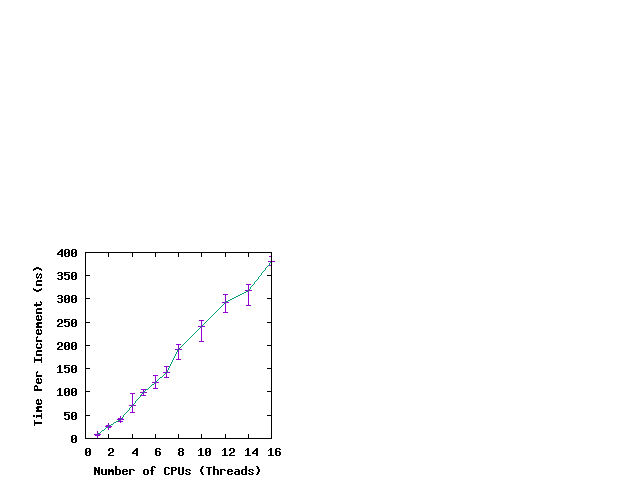
\includegraphics{CodeSamples/count/atomic_nehalem.pdf}}
\caption{Atomic Increment Scalability on Nehalem}
\label{fig:count:Atomic Increment Scalability on Nehalem}
\end{figure}

The straightforward way to count accurately is to use atomic operations,
as shown in
Listing~\ref{lst:count:Just Count Atomically!} (\path{count_atomic.c}).
\begin{lineref}[ln:count:count_atomic:inc-read]
Line~\lnref{counter} defines an atomic variable,
line~\lnref{inc} atomically increments it, and
line~\lnref{read} reads it out.
\end{lineref}
Because this is atomic, it keeps perfect count.
However, it is slower: on a Intel Core Duo laptop, it is about
six times slower than non-atomic increment
when a single thread is incrementing, and more than \emph{ten times}
slower if two threads are incrementing.\footnote{
	Interestingly enough, a pair of threads non-atomically incrementing
	a counter will cause the counter to increase more quickly than
	a pair of threads atomically incrementing the counter.
	Of course, if your only goal is to make the counter increase
	quickly, an easier approach is to simply assign a large value
	to the counter.
	Nevertheless, there is likely to be a role for algorithms that
	use carefully relaxed notions of correctness in order to gain
	greater performance and
	scalability~\cite{Andrews91textbook,Arcangeli03,DavidUngar2011unsync}.}

This poor performance should not be a surprise, given the discussion in
Chapter~\ref{chp:Hardware and its Habits},
nor should it be a surprise that the performance of atomic increment
gets slower as the number of CPUs and threads increase, as shown in
Figure~\ref{fig:count:Atomic Increment Scalability on Nehalem}.
In this figure, the horizontal dashed line resting on the x~axis
is the ideal performance that would be achieved
by a perfectly scalable algorithm: with such an algorithm, a given
increment would incur the same overhead that it would in a single-threaded
program.
Atomic increment of a single global variable is clearly
decidedly non-ideal, and gets worse as you add CPUs.

\QuickQuiz{}
	Why doesn't the dashed line on the x~axis meet the 
	diagonal line at $x=1$?
\QuickQuizAnswer{
	Because of the overhead of the atomic operation.
	The dashed line on the x~axis represents the overhead of
	a single \emph{non-atomic} increment.
	After all, an \emph{ideal} algorithm would not only scale
	linearly, it would also incur no performance penalty compared
	to single-threaded code.

	This level of idealism may seem severe, but if it is good
	enough for Linus Torvalds, it is good enough for you.
} \QuickQuizEnd

\QuickQuiz{}
	But atomic increment is still pretty fast.
	And incrementing a single variable in a tight loop sounds
	pretty unrealistic to me, after all, most of the program's
	execution should be devoted to actually doing work, not accounting
	for the work it has done!
	Why should I care about making this go faster?
\QuickQuizAnswer{
	In many cases, atomic increment will in fact be fast enough
	for you.
	In those cases, you should by all means use atomic increment.
	That said, there are many real-world situations where
	more elaborate counting algorithms are required.
	The canonical example of such a situation is counting packets
	and bytes in highly optimized networking stacks, where it is
	all too easy to find much of the execution time going into
	these sorts of accounting tasks, especially on large
	multiprocessors.

	In addition, as noted at the beginning of this chapter,
	counting provides an excellent view of the
	issues encountered in shared-memory parallel programs.
} \QuickQuizEnd

\begin{figure}[tb]
\centering
\resizebox{3in}{!}{\includegraphics{count/GlobalInc}}
\caption{Data Flow For Global Atomic Increment}
\label{fig:count:Data Flow For Global Atomic Increment}
\end{figure}

\begin{figure}[tb]
\centering
\resizebox{3.2in}{!}{\includegraphics{cartoons/r-2014-One-one-thousand}}
\caption{Waiting to Count}
\ContributedBy{Figure}{fig:count:Waiting to Count}{Melissa Broussard}
\end{figure}

For another perspective on global atomic increment, consider
Figure~\ref{fig:count:Data Flow For Global Atomic Increment}.
In order for each CPU to get a chance to increment a given
global variable, the cache line containing that variable must
circulate among all the CPUs, as shown by the red arrows.
Such circulation will take significant time, resulting in
the poor performance seen in
Figure~\ref{fig:count:Atomic Increment Scalability on Nehalem},
which might be thought of as shown in
Figure~\ref{fig:count:Waiting to Count}.
The following sections discuss high-performance counting, which
avoids the delays inherent in such circulation.

\QuickQuiz{}
	But why can't CPU designers simply ship the addition operation to the
	data, avoiding the need to circulate the cache line containing
	the global variable being incremented?
\QuickQuizAnswer{
	It might well be possible to do this in some cases.
	However, there are a few complications:
	\begin{enumerate}
	\item	If the value of the variable is required, then the
		thread will be forced to wait for the operation
		to be shipped to the data, and then for the result
		to be shipped back.
	\item	If the atomic increment must be ordered with respect
		to prior and/or subsequent operations, then the thread
		will be forced to wait for the operation to be shipped
		to the data, and for an indication that the operation
		completed to be shipped back.
	\item	Shipping operations among CPUs will likely require
		more lines in the system interconnect, which will consume
		more die area and more electrical power.
	\end{enumerate}
	But what if neither of the first two conditions holds?
	Then you should think carefully about the algorithms discussed
	in Section~\ref{sec:count:Statistical Counters}, which achieve
	near-ideal performance on commodity hardware.

\begin{figure}[tb]
\centering
\resizebox{3in}{!}{\includegraphics{count/GlobalTreeInc}}
\caption{Data Flow For Global Combining-Tree Atomic Increment}
\label{fig:count:Data Flow For Global Combining-Tree Atomic Increment}
\end{figure}

	If either or both of the first two conditions hold, there is
	\emph{some} hope for improved hardware.
	One could imagine the hardware implementing a combining tree,
	so that the increment requests from multiple CPUs are combined
	by the hardware into a single addition when the combined request
	reaches the hardware.
	The hardware could also apply an order to the requests, thus
	returning to each CPU the return value corresponding to its
	particular atomic increment.
	This results in instruction latency that varies as $\O{\log N}$,
	where $N$ is the number of CPUs, as shown in
	Figure~\ref{fig:count:Data Flow For Global Combining-Tree Atomic Increment}.
	And CPUs with this sort of hardware optimization are starting to
	appear as of 2011.

	This is a great improvement over the $\O{N}$ performance
	of current hardware shown in
	Figure~\ref{fig:count:Data Flow For Global Atomic Increment},
	and it is possible that hardware latencies might decrease
	further if innovations such as three-dimensional fabrication prove
	practical.
	Nevertheless, we will see that in some important special cases,
	software can do \emph{much} better.
} \QuickQuizEnd

\section{Statistical Counters}
\label{sec:count:Statistical Counters}
%
\epigraph{Facts are stubborn things, but statistics are pliable.}
	 {\emph{Mark Twain}}

This section covers the common special case of statistical counters, where
the count is updated extremely frequently and the value is read out
rarely, if ever.
These will be used to solve the network-packet counting problem
posed in \QuickQuizRef{\QcountQstatcnt}.

\subsection{Design}

Statistical counting is typically handled by providing a counter per
thread (or CPU, when running in the kernel), so that each thread
updates its own counter, as was foreshadowed in
Section~\ref{sec:toolsoftrade:Per-CPU Variables}.
The aggregate value of the counters is read out by simply summing up
all of the threads' counters,
relying on the commutative and associative properties of addition.
This is an example of the Data Ownership pattern that will be introduced in
Section~\ref{sec:SMPdesign:Data Ownership}.

\QuickQuiz{}
	But doesn't the fact that C's ``integers'' are limited in size
	complicate things?
\QuickQuizAnswer{
	No, because modulo addition is still commutative and associative.
	At least as long as you use unsigned integers.
	Recall that in the C standard, overflow of signed integers results
	in undefined behavior, never mind the fact that machines that
	do anything other than wrap on overflow are quite rare these days.
	Unfortunately, compilers frequently carry out optimizations that
	assume that signed integers will not overflow, so if your code
	allows signed integers to overflow, you can run into trouble
	even on twos-complement hardware.

	That said, one potential source of additional complexity arises
	when attempting to gather (say) a 64-bit sum from 32-bit
	per-thread counters.
	Dealing with this added complexity is left as
	an exercise for the reader, for whom some of the techniques
	introduced later in this chapter could be quite helpful.
} \QuickQuizEnd

\subsection{Array-Based Implementation}
\label{sec:count:Array-Based Implementation}

One way to provide per-thread variables is to allocate an array with
one element per
thread (presumably cache aligned and padded to avoid false sharing).

\QuickQuiz{}
	An array???
	But doesn't that limit the number of threads?
\QuickQuizAnswer{
	It can, and in this toy implementation, it does.
	But it is not that hard to come up with an alternative
	implementation that permits an arbitrary number of threads,
	for example, using \GCC's \co{__thread} facility,
	as shown in
	Section~\ref{sec:count:Per-Thread-Variable-Based Implementation}.
} \QuickQuizEnd

\begin{listing}[tbp]
\input{CodeSamples/count/count_stat@inc-read.fcv}
\caption{Array-Based Per-Thread Statistical Counters}
\label{lst:count:Array-Based Per-Thread Statistical Counters}
\end{listing}

Such an array can be wrapped into per-thread primitives, as shown in
Listing~\ref{lst:count:Array-Based Per-Thread Statistical Counters}
(\path{count_stat.c}).
\begin{lineref}[ln:count:count_stat:inc-read]
Line~\lnref{define} defines an array containing a set of per-thread counters of
type \co{unsigned long} named, creatively enough, \co{counter}.

Lines~\lnref{inc:b}-\lnref{inc:e}
show a function that increments the counters, using the
\co{__get_thread_var()} primitive to locate the currently running
thread's element of the \co{counter} array.
Because this element is modified only by the corresponding thread,
non-atomic increment suffices.
However, this code uses \co{WRITE_ONCE()} to prevent destructive compiler
optimizations.
For but one example, the compiler is within its rights to use a
to-be-stored-to location as temporary storage, thus writing what
would be for all intents and purposes garbage to that location
just before doing the desired store.
This could of course be rather confusing to anything attempting to
read out the count.
The use of \co{WRITE_ONCE()} prevents this optimization and others besides.

\QuickQuiz{}
	What other nasty optimizations could \GCC\ apply?
\QuickQuizAnswer{
	According to the C standard, the effects of doing a normal store
	to a variable that might be concurrently loaded by some other
	thread are undefined.
	It turns out that the C standard really has no other choice,
	given that C must support (for example) eight-bit architectures
	which are incapable of atomically loading a \co{long}.
	Recent versions of the C standard have introduced atomics, which
	are intended to fill this gap.
	However, an attempt to apply them to the Linux kernel gave
	at best mixed results~\cite{JonathanCorbet2016C11atomics},
	in part due to the poor quality of code emitted for atomics.
	In addition, the Linux kernel expects much more from its
	memory model than C11 atomics provide, including control
	dependencies, full barriers/fences, and low-overhead address
	and data dependencies~\cite{PaulEMcKenney2016P0124R5-LKMM}.

	At some point, C11 atomics might close these gaps,
	but until then, the Linux kernel uses a combination of
	volatile accesses, inline assembly, compiler directives,
	and coding standards to safely access shared variables.
	This approach allows the Linux kernel to maintain excellent
	performance and also to make good use of older compilers
	that do not support C11 atomics, however, it also requires
	some effort to port the Linux kernel to a new CPU architecture.
	That said, significant effort would be required even if C11
	atomics could be used directly due to the need to handle context
	switches, interrupts, exceptions, memory-management units,
	power control for energy efficiency, and much else besides.
	It is therefore reasonable to expect that any Linux-kernel
	adoption of C11 atomics will be incremental at best.

	But if the code is doing loads and stores that the underlying
	hardware can implement with single instructions, why not just
	use plain old C-language assignment statements to access shared
	variables?
	The problem is that the compiler is within its rights to assume
	that no other thread is modifying the variable being accessed.
	Given a plain old C-language load, the compiler would therefore
	be within its rights to do the load byte at a time
	(``load tearing''), repeat the load (popular if register
	pressure is high), or fuse a pair of consecutive loads from
	the same variable.
	Given a plain old C-language store, the compiler would be within
	its rights to do the store byte at a time (``store tearing''),
	invent a store (for example, using the stored-to variable as
	a temporary just prior to the intended store), or omit a store
	in favor of a later store to the same variable.
	Although each of these actions would preserve the correctness
	of a single-threaded algorithm, any of them could easily destroy
	the correctness of a concurrent algorithm.
	Given a major tenet of shared-memory concurrency is to support
	such conflicting accesses, it is quite unwise to use normal
	C-language loads and stores when accessing variables that might
	be concurrently updated by other threads.
	Further, given that current C11 atomics are not (yet?) a good
	match for the Linux kernel, something else is required.

	One approach is to prevent concurrent updates by using
	blocking synchronization primitives such as locking
	(see Chapter~\ref{chp:Locking}).
	Alternatively, volatile accesses may be used, such as those provided
	by \co{READ_ONCE()} and \co{WRITE_ONCE()},\footnote{
		Simple definitions of \co{READ_ONCE()} and
		\co{WRITE_ONCE()} are shown in
		Listing~\ref{lst:toolsoftrade:Compiler Barrier Primitive (for GCC)}.}
	at least in cases where the hardware is capable of accessing
	the value with a single memory-reference instruction.
	However, volatile accesses do not by themselves suffice for
	high-performance and reliable synchronization mechanisms.
	The Linux kernel therefore combines volatile accesses with
	the aforementioned inline assembly, compiler directives, and
	coding standards.
} \QuickQuizEnd

Lines~\lnref{read:b}-\lnref{read:e}
show a function that reads out the aggregate value of the counter,
using the \co{for_each_thread()} primitive to iterate over the list of
currently running threads, and using the \co{per_thread()} primitive
to fetch the specified thread's counter.
This code also uses \co{READ_ONCE()} to ensure that the compiler doesn't
optimize these loads into oblivion.
For but one example, a pair of consecutive calls to \co{read_count()}
might be inlined, and an intrepid optimizer might notice that the same
locations were being summed and thus incorrectly conclude that it would
be simply wonderful to sum them once and use the resulting value twice.
This sort of optimization might be rather frustrating to people expecting
later \co{read_count()} calls to return larger values.
The use of \co{READ_ONCE()} prevents this optimization and others besides.
\end{lineref}

\QuickQuiz{}
	How does the per-thread \co{counter} variable in
	Listing~\ref{lst:count:Array-Based Per-Thread Statistical Counters}
	get initialized?
\QuickQuizAnswer{
	The C standard specifies that the initial value of
	global variables is zero, unless they are explicitly initialized.
	So the initial value of all the instances of \co{counter}
	will be zero.
	Furthermore, in the common case where the user is interested only
	in differences between consecutive reads
	from statistical counters, the initial value is irrelevant.
} \QuickQuizEnd

\QuickQuiz{}
	How is the code in
	Listing~\ref{lst:count:Array-Based Per-Thread Statistical Counters}
	supposed to permit more than one counter?
\QuickQuizAnswer{
	Indeed, this toy example does not support more than one counter.
	Modifying it so that it can provide multiple counters is left
	as an exercise to the reader.
} \QuickQuizEnd

\begin{figure}[tb]
\centering
\resizebox{3in}{!}{\includegraphics{count/PerThreadInc}}
\caption{Data Flow For Per-Thread Increment}
\label{fig:count:Data Flow For Per-Thread Increment}
\end{figure}

This approach scales linearly with increasing number of updater threads
invoking \co{inc_count()}.
As is shown by the green arrows on each CPU in
Figure~\ref{fig:count:Data Flow For Per-Thread Increment},
the reason for this is that each CPU can make rapid progress incrementing
its thread's variable, without any expensive cross-system communication.
As such, this section solves the network-packet counting problem presented
at the beginning of this chapter.

\QuickQuiz{}
	The read operation takes time to sum up the per-thread values,
	and during that time, the counter could well be changing.
	This means that the value returned by
	\co{read_count()} in
	Listing~\ref{lst:count:Array-Based Per-Thread Statistical Counters}
	will not necessarily be exact.
	Assume that the counter is being incremented at rate
	$r$ counts per unit time, and that \co{read_count()}'s
	execution consumes $\Delta$ units of time.
	What is the expected error in the return value?
\QuickQuizAnswer{
	Let's do worst-case analysis first, followed by a less
	conservative analysis.

	In the worst case, the read operation completes immediately,
	but is then delayed for $\Delta$ time units before returning,
	in which case the worst-case error is simply $r \Delta$.

	This worst-case behavior is rather unlikely, so let us instead
	consider the case where the reads from each of the $N$
	counters is spaced equally over the time period $\Delta$.
	There will be $N+1$ intervals of duration $\frac{\Delta}{N+1}$
	between the $N$ reads.
	The error due to the delay after the read from the last thread's
	counter will be given by $\frac{r \Delta}{N \left( N + 1 \right)}$,
	the second-to-last thread's counter by
	$\frac{2 r \Delta}{N \left( N + 1 \right)}$,
	the third-to-last by
	$\frac{3 r \Delta}{N \left( N + 1 \right)}$,
	and so on.
	The total error is given by the sum of the errors due to the
	reads from each thread's counter, which is:

	\begin{equation}
		\frac{r \Delta}{N \left( N + 1 \right)}
			\sum_{i = 1}^N i
	\end{equation}

	Expressing the summation in closed form yields:

	\begin{equation}
		\frac{r \Delta}{N \left( N + 1 \right)}
			\frac{N \left( N + 1 \right)}{2}
	\end{equation}

	Cancelling yields the intuitively expected result:

	\begin{equation}
		\frac{r \Delta}{2}
	\label{eq:count:CounterErrorAverage}
	\end{equation}

	It is important to remember that error continues accumulating
	as the caller executes code making use of the count returned
	by the read operation.
	For example, if the caller spends time $t$ executing some
	computation based on the result of the returned count, the
	worst-case error will have increased to $r \left(\Delta + t\right)$.

	The expected error will have similarly increased to:

	\begin{equation}
		r \left( \frac{\Delta}{2} + t \right)
	\end{equation}

	Of course, it is sometimes unacceptable for the counter to
	continue incrementing during the read operation.
	Section~\ref{sec:count:Applying Exact Limit Counters}
	discusses a way to handle this situation.

	Thus far, we have been considering a counter that is only
	increased, never decreased.
	If the counter value is being changed by $r$ counts per unit
	time, but in either direction, we should expect the error
	to reduce.
	However, the worst case is unchanged because although the
	counter \emph{could} move in either direction, the worst
	case is when the read operation completes immediately,
	but then is delayed for $\Delta$ time units, during which
	time all the changes in the counter's value move it in
	the same direction, again giving us an absolute error
	of $r \Delta$.

	There are a number of ways to compute the average error,
	based on a variety of assumptions about the patterns of
	increments and decrements.
	For simplicity, let's assume that the $f$ fraction of
	the operations are decrements, and that the error of interest
	is the deviation from the counter's long-term trend line.
	Under this assumption, if $f$ is less than or equal to 0.5,
	each decrement will be cancelled by an increment, so that
	$2f$ of the operations will cancel each other, leaving
	$1-2f$ of the operations being uncancelled increments.
	On the other hand, if $f$ is greater than 0.5, $1-f$ of
	the decrements are cancelled by increments, so that the
	counter moves in the negative direction by $-1+2\left(1-f\right)$,
	which simplifies to $1-2f$, so that the counter moves an average
	of $1-2f$ per operation in either case.
	Therefore, that the long-term
	movement of the counter is given by $\left( 1-2f \right) r$.
	Plugging this into
	Equation~\ref{eq:count:CounterErrorAverage} yields:

	\begin{equation}
		\frac{\left( 1 - 2 f \right) r \Delta}{2}
	\end{equation}

	All that aside, in most uses of statistical counters, the
	error in the value returned by \co{read_count()} is
	irrelevant.
	This irrelevance is due to the fact that the time required
	for \co{read_count()} to execute is normally extremely
	small compared to the time interval between successive
	calls to \co{read_count()}.
} \QuickQuizEnd

However, this excellent update-side scalability comes at great read-side
expense for large numbers of threads.
The next section shows one way to reduce read-side expense while
still retaining the update-side scalability.

\subsection{Eventually Consistent Implementation}
\label{sec:count:Eventually Consistent Implementation}

One way to retain update-side scalability while greatly improving
read-side performance is to weaken consistency requirements.
The counting algorithm in the previous section is guaranteed to
return a value between the value that an ideal counter would have
taken on near the beginning of \co{read_count()}'s execution and
that near the end of \co{read_count()}'s execution.
\emph{Eventual consistency}~\cite{WernerVogels:2009:EventuallyConsistent}
provides a weaker
guarantee: in absence of calls to \co{inc_count()}, calls to
\co{read_count()} will eventually return an accurate count.

We exploit eventual consistency by maintaining a global counter.
However, updaters only manipulate their per-thread counters.
A separate thread is provided to transfer counts from the per-thread
counters to the global counter.
Readers simply access the value of the global counter.
If updaters are active, the value used by the readers will be out of
date, however, once updates cease, the global counter will eventually
converge on the true value---hence this approach qualifies as
eventually consistent.

\begin{listing}[tbp]
\input{CodeSamples/count/count_stat_eventual@whole.fcv}
\caption{Array-Based Per-Thread Eventually Consistent Counters}
\label{lst:count:Array-Based Per-Thread Eventually Consistent Counters}
\end{listing}

\begin{lineref}[ln:count:count_stat_eventual:whole]
The implementation is shown in
Listing~\ref{lst:count:Array-Based Per-Thread Eventually Consistent Counters}
(\path{count_stat_eventual.c}).
Lines~\lnref{per_thr_cnt}-\lnref{glb_cnt}
show the per-thread variable and the global variable that
track the counter's value, and line~\lnref{stopflag} shows \co{stopflag}
which is used to coordinate termination (for the case where we want
to terminate the program with an accurate counter value).
The \co{inc_count()} function shown on
lines~\lnref{inc:b}-\lnref{inc:e} is similar to its
counterpart in
Listing~\ref{lst:count:Array-Based Per-Thread Statistical Counters}.
The \co{read_count()} function shown on
lines~\lnref{read:b}-\lnref{read:e} simply returns the
value of the \co{global_count} variable.

However, the \co{count_init()} function on
lines~\lnref{init:b}-\lnref{init:e}
creates the \co{eventual()} thread shown on
lines~\lnref{eventual:b}-\lnref{eventual:e}, which
cycles through all the threads,
summing the per-thread local \co{counter} and storing the
sum to the \co{global_count} variable.
The \co{eventual()} thread waits an arbitrarily chosen one millisecond
between passes.
The \co{count_cleanup()} function on
lines~\lnref{cleanup:b}-\lnref{cleanup:e} coordinates termination.

This approach gives extremely fast counter read-out while still
supporting linear counter-update performance.
However, this excellent read-side performance and update-side scalability
comes at the cost of the additional thread running \co{eventual()}.
\end{lineref}

\QuickQuiz{}
	Why doesn't \co{inc_count()} in
	Listing~\ref{lst:count:Array-Based Per-Thread Eventually Consistent Counters}
	need to use atomic instructions?
	After all, we now have multiple threads accessing the per-thread
	counters!
\QuickQuizAnswer{
	Because one of the two threads only reads, and because the
	variable is aligned and machine-sized, non-atomic instructions
	suffice.
	That said, the \co{READ_ONCE()} macro is used to prevent
	compiler optimizations that might otherwise prevent the
	counter updates from becoming visible to
	\co{eventual()}.\footnote{
		A simple definition of \co{READ_ONCE()} is shown in
		Listing~\ref{lst:toolsoftrade:Compiler Barrier Primitive (for GCC)}.}

	An older version of this algorithm did in fact use atomic
	instructions, kudos to Ersoy Bayramoglu for pointing out that
	they are in fact unnecessary.
	That said, atomic instructions would be needed in cases where
	the per-thread \co{counter} variables were smaller than the
	global \co{global_count}.
	However, note that on a 32-bit system,
	the per-thread \co{counter} variables
	might need to be limited to 32 bits in order to sum them accurately,
	but with a 64-bit \co{global_count} variable to avoid overflow.
	In this case, it is necessary to zero the per-thread
	\co{counter} variables periodically in order to avoid overflow.
	It is extremely important to note that this zeroing cannot
	be delayed too long or overflow of the smaller per-thread
	variables will result.
	This approach therefore imposes real-time requirements on the
	underlying system, and in turn must be used with extreme care.

	In contrast, if all variables are the same size, overflow
	of any variable is harmless because the eventual sum
	will be modulo the word size.
} \QuickQuizEnd

\QuickQuiz{}
	Won't the single global thread in the function \co{eventual()} of
	Listing~\ref{lst:count:Array-Based Per-Thread Eventually Consistent Counters}
	be just as severe a bottleneck as a global lock would be?
\QuickQuizAnswer{
	In this case, no.
	What will happen instead is that as the number of threads increases,
	the estimate of the counter
	value returned by \co{read_count()} will become more inaccurate.
} \QuickQuizEnd

\QuickQuiz{}
	Won't the estimate returned by \co{read_count()} in
	Listing~\ref{lst:count:Array-Based Per-Thread Eventually Consistent Counters}
	become increasingly
	inaccurate as the number of threads rises?
\QuickQuizAnswer{
	Yes.
	If this proves problematic, one fix is to provide multiple
	\co{eventual()} threads, each covering its own subset of
	the other threads.
	In more extreme cases, a tree-like hierarchy of
	\co{eventual()} threads might be required.
} \QuickQuizEnd

\QuickQuiz{}
	Given that in the eventually\-/consistent algorithm shown in
	Listing~\ref{lst:count:Array-Based Per-Thread Eventually Consistent Counters}
	both reads and updates have extremely low overhead
	and are extremely scalable, why would anyone bother with the
	implementation described in
	Section~\ref{sec:count:Array-Based Implementation},
	given its costly read-side code?
\QuickQuizAnswer{
	The thread executing \co{eventual()} consumes CPU time.
	As more of these eventually\-/consistent counters are added,
	the resulting \co{eventual()} threads will eventually
	consume all available CPUs.
	This implementation therefore suffers a different sort of
	scalability limitation, with the scalability limit being in
	terms of the number of eventually consistent counters rather
	than in terms of the number of threads or CPUs.

	Of course, it is possible to make other tradeoffs.
	For example, a single thread could be created to handle all
	eventually\-/consistent counters, which would limit the
	overhead to a single CPU, but would result in increasing
	update-to-read latencies as the number of counters increased.
	Alternatively, that single thread could track the update rates
	of the counters, visiting the frequently\-/updated counters
	more frequently.
	In addition, the number of threads handling the counters could
	be set to some fraction of the total number of CPUs, and
	perhaps also adjusted at runtime.
	Finally, each counter could specify its latency, and
	deadline\-/scheduling techniques could be used to provide
	the required latencies to each counter.

	There are no doubt many other tradeoffs that could be made.
} \QuickQuizEnd

\subsection{Per-Thread-Variable-Based Implementation}
\label{sec:count:Per-Thread-Variable-Based Implementation}
\NoIndentAfterThis

\begin{listing}[tb]
\input{CodeSamples/count/count_end@whole.fcv}
\caption{Per-Thread Statistical Counters}
\label{lst:count:Per-Thread Statistical Counters}
\end{listing}

Fortunately, \GCC\ provides an \co{__thread} storage class that provides
per-thread storage.
This can be used as shown in
Listing~\ref{lst:count:Per-Thread Statistical Counters} (\path{count_end.c})
to implement
a statistical counter that not only scales, but that also incurs little
or no performance penalty to incrementers compared to simple non-atomic
increment.

\begin{lineref}[ln:count:count_end:whole]
Lines~\lnref{var:b}-\lnref{var:e} define needed variables:
\co{counter} is the per-thread counter
variable, the \co{counterp[]} array allows threads to access each others'
counters, \co{finalcount} accumulates the total as individual threads exit,
and \co{final_mutex} coordinates between threads accumulating the total
value of the counter and exiting threads.
\end{lineref}

\QuickQuiz{}
	Why do we need an explicit array to find the other threads'
	counters?
	Why doesn't \GCC\ provide a \co{per_thread()} interface, similar
	to the Linux kernel's \co{per_cpu()} primitive, to allow
	threads to more easily access each others' per-thread variables?
\QuickQuizAnswer{
	Why indeed?

	To be fair, \GCC\ faces some challenges that the Linux kernel
	gets to ignore.
	When a user-level thread exits, its per-thread variables all
	disappear, which complicates the problem of per-thread-variable
	access, particularly before the advent of user-level RCU
	(see Section~\ref{sec:defer:Read-Copy Update (RCU)}).
	In contrast, in the Linux kernel, when a CPU goes offline,
	that CPU's per-CPU variables remain mapped and accessible.

	Similarly, when a new user-level thread is created, its
	per-thread variables suddenly come into existence.
	In contrast, in the Linux kernel, all per-CPU variables are
	mapped and initialized at boot time, regardless of whether
	the corresponding CPU exists yet, or indeed, whether the
	corresponding CPU will ever exist.

	A key limitation that the Linux kernel imposes is a compile-time
	maximum bound on the number of CPUs, namely, \co{CONFIG_NR_CPUS},
	along with a typically tighter boot-time bound of \co{nr_cpu_ids}.
	In contrast, in user space, there is no hard-coded upper limit
	on the number of threads.

	Of course, both environments must handle dynamically loaded
	code (dynamic libraries in user space, kernel modules in the
	Linux kernel), which increases the complexity of per-thread
	variables.

	These complications make it significantly harder for user-space
	environments to provide access to other threads' per-thread
	variables.
	Nevertheless, such access is highly useful, and it is hoped
	that it will someday appear.
} \QuickQuizEnd

\begin{lineref}[ln:count:count_end:whole:inc]
The \co{inc_count()} function used by updaters is quite simple, as can
be seen on lines~\lnref{b}-\lnref{e}.
\end{lineref}

\begin{lineref}[ln:count:count_end:whole:read]
The \co{read_count()} function used by readers is a bit more complex.
Line~\lnref{acquire} acquires a lock to exclude exiting threads, and
line~\lnref{release} releases it.
Line~\lnref{sum:init} initializes the sum to the count accumulated by those threads that
have already exited, and
lines~\lnref{loop:b}-\lnref{loop:e} sum the counts being accumulated
by threads currently running.
Finally, line~\lnref{return} returns the sum.
\end{lineref}

\QuickQuiz{}
	\begin{lineref}[ln:count:count_end:whole:read]
	Doesn't the check for \co{NULL} on line~\lnref{check} of
	Listing~\ref{lst:count:Per-Thread Statistical Counters}
	add extra branch mispredictions?
	Why not have a variable set permanently to zero, and point
	unused counter-pointers to that variable rather than setting
	them to \co{NULL}?
	\end{lineref}
\QuickQuizAnswer{
	This is a reasonable strategy.
	Checking for the performance difference is left as an exercise
	for the reader.
	However, please keep in mind that the fastpath is not
	\co{read_count()}, but rather \co{inc_count()}.
} \QuickQuizEnd

\QuickQuiz{}
	Why on earth do we need something as heavyweight as a \emph{lock}
	guarding the summation in the function \co{read_count()} in
	Listing~\ref{lst:count:Per-Thread Statistical Counters}?
\QuickQuizAnswer{
	Remember, when a thread exits, its per-thread variables disappear.
	Therefore, if we attempt to access a given thread's per-thread
	variables after that thread exits, we will get a segmentation
	fault.
	The lock coordinates summation and thread exit, preventing this
	scenario.

	Of course, we could instead read-acquire a reader-writer lock,
	but Chapter~\ref{chp:Deferred Processing} will introduce even
	lighter-weight mechanisms for implementing the required coordination.

	Another approach would be to use an array instead of a per-thread
	variable, which, as Alexey Roytman notes, would eliminate
	the tests against \co{NULL}.
	However, array accesses are often slower than accesses to
	per-thread variables, and use of an array would imply a
	fixed upper bound on the number of threads.
	Also, note that neither tests nor locks are needed on the
	\co{inc_count()} fastpath.
} \QuickQuizEnd

\begin{lineref}[ln:count:count_end:whole:reg]
Lines~\lnref{b}-\lnref{e} show the \co{count_register_thread()}
function, which
must be called by each thread before its first use of this counter.
This function simply sets up this thread's element of the \co{counterp[]}
array to point to its per-thread \co{counter} variable.
\end{lineref}

\QuickQuiz{}
	Why on earth do we need to acquire the lock in
	\co{count_register_thread()} in
	Listing~\ref{lst:count:Per-Thread Statistical Counters}?
	It is a single properly aligned machine-word store to a location
	that no other thread is modifying, so it should be atomic anyway,
	right?
\QuickQuizAnswer{
	This lock could in fact be omitted, but better safe than
	sorry, especially given that this function is executed only at
	thread startup, and is therefore not on any critical path.
	Now, if we were testing on machines with thousands of CPUs,
	we might need to omit the lock, but on machines with ``only''
	a hundred or so CPUs, there is no need to get fancy.
} \QuickQuizEnd

\begin{lineref}[ln:count:count_end:whole:unreg]
Lines~\lnref{b}-\lnref{e} show the \co{count_unregister_thread()}
function, which
must be called prior to exit by each thread that previously called
\co{count_register_thread()}.
Line~\lnref{acquire} acquires the lock, and
line~\lnref{release} releases it, thus excluding any
calls to \co{read_count()} as well as other calls to
\co{count_unregister_thread()}.
Line~\lnref{add} adds this thread's \co{counter} to the global
\co{finalcount},
and then line~\lnref{NULL} \co{NULL}s out its \co{counterp[]} array entry.
A subsequent call to \co{read_count()} will see the exiting thread's
count in the global \co{finalcount}, and will skip the exiting thread
when sequencing through the \co{counterp[]} array, thus obtaining
the correct total.
\end{lineref}

This approach gives updaters almost exactly the same performance as
a non-atomic add, and also scales linearly.
On the other hand, concurrent reads contend for a single global lock,
and therefore perform poorly and scale abysmally.
However, this is not a problem for statistical counters, where incrementing
happens often and readout happens almost never.
Of course, this approach is considerably more complex than the
array-based scheme, due to the fact that a given thread's per-thread
variables vanish when that thread exits.

\QuickQuiz{}
	Fine, but the Linux kernel doesn't have to acquire a lock
	when reading out the aggregate value of per-CPU counters.
	So why should user-space code need to do this???
\QuickQuizAnswer{
	Remember, the Linux kernel's per-CPU variables are always
	accessible, even if the corresponding CPU is offline---even
	if the corresponding CPU never existed and never will exist.

\begin{listing}[tb]
\input{CodeSamples/count/count_tstat@whole.fcv}
\caption{Per-Thread Statistical Counters With Lockless Summation}
\label{lst:count:Per-Thread Statistical Counters With Lockless Summation}
\end{listing}

	One workaround is to ensure that each thread continues to exist
	until all threads are finished, as shown in
	Listing~\ref{lst:count:Per-Thread Statistical Counters With Lockless Summation}
	(\path{count_tstat.c}).
	Analysis of this code is left as an exercise to the reader,
	however, please note that it requires tweaks in the
	\path{counttorture.h} counter-evaluation scheme.
	(Hint: See \co{#ifndef KEEP_GCC_THREAD_LOCAL}.)
	Chapter~\ref{chp:Deferred Processing} will introduce 
	synchronization mechanisms that handle this situation in a much
	more graceful manner.
} \QuickQuizEnd

\subsection{Discussion}

These three implementations show that it is possible to obtain uniprocessor
performance for statistical counters, despite running on a parallel
machine.

\QuickQuiz{}
	What fundamental difference is there between counting packets
	and counting the total number of bytes in the packets, given
	that the packets vary in size?
\QuickQuizAnswer{
	When counting packets, the counter is only incremented by the
	value one.
	On the other hand, when counting bytes, the counter might
	be incremented by largish numbers.

	Why does this matter?
	Because in the increment-by-one case, the value returned will
	be exact in the sense that the counter must necessarily have
	taken on that value at some point in time, even if it is impossible
	to say precisely when that point occurred.
	In contrast, when counting bytes, two different threads might
	return values that are inconsistent with any global ordering
	of operations.

	To see this, suppose that thread~0 adds the value three to its
	counter, thread~1 adds the value five to its counter, and
	threads~2 and 3 sum the counters.
	If the system is ``weakly ordered'' or if the compiler
	uses aggressive optimizations, thread~2 might find the
	sum to be three and thread~3 might find the sum to be five.
	The only possible global orders of the sequence of values
	of the counter are 0,3,8 and 0,5,8, and neither order is
	consistent with the results obtained.

	If you missed this one, you are not alone.
	Michael Scott used this question to stump Paul E.~McKenney
	during Paul's Ph.D. defense.
} \QuickQuizEnd

\QuickQuiz{}
	Given that the reader must sum all the threads' counters,
	this could take a long time given large numbers of threads.
	Is there any way that the increment operation can remain
	fast and scalable while allowing readers to also enjoy
	reasonable performance and scalability?
\QuickQuizAnswer{
	One approach would be to maintain a global approximation
	to the value.
	Updaters would increment their per-thread variable, but when it
	reached some predefined limit, atomically add it to a global
	variable, then zero their per-thread variable.
	This would permit a tradeoff between average increment overhead
	and accuracy of the value read out.

	The reader is encouraged to think up and try out other approaches,
	for example, using a combining tree.
} \QuickQuizEnd

Given what has been presented in this section, you should now be able
to answer the Quick Quiz about statistical counters for networking
near the beginning of this chapter.

\section{Approximate Limit Counters}
\label{sec:count:Approximate Limit Counters}
%
\epigraph{An approximate answer to the right problem is worth a good deal
	  more than an exact answer to an approximate problem.}
	 {\emph{John Tukey}}

Another special case of counting involves limit-checking.
For example, as noted in the approximate structure-allocation limit
problem in \QuickQuizRef{\QcountQapproxcnt},
suppose that you need to maintain a count of the number of
structures allocated in order to fail any allocations once the number
of structures in use exceeds a limit, in this case, 10,000.
Suppose further that these structures are short-lived, that this
limit is rarely exceeded, and that this limit is approximate in
that it is OK to exceed it sometimes by some bounded amount
(see Section~\ref{sec:count:Exact Limit Counters}
if you instead need the limit to be exact).

\subsection{Design}

One possible design for limit counters is to divide the limit of 10,000
by the number of threads, and give each thread a fixed pool of structures.
For example, given 100 threads, each thread would manage its own pool
of 100 structures.
This approach is simple, and in some cases works well, but it does not
handle the common case where a given structure is allocated by one
thread and freed by another~\cite{McKenney93}.
On the one hand, if a given thread takes credit for any structures it
frees, then the thread doing most of the allocating runs out
of structures, while the threads doing most of the freeing have lots
of credits that they cannot use.
On the other hand, if freed structures are credited to the CPU that
allocated them, it will be necessary for CPUs to manipulate each
others' counters, which will require expensive atomic instructions
or other means of communicating between threads.\footnote{
	That said, if each structure will always be freed
	by the same CPU (or thread) that allocated it, then
	this simple partitioning approach works extremely well.}

In short, for many important workloads, we cannot fully partition the counter.
Given that partitioning the counters was what brought the excellent
update-side performance for the three schemes discussed in
Section~\ref{sec:count:Statistical Counters}, this might be grounds
for some pessimism.
However, the eventually consistent algorithm presented in
Section~\ref{sec:count:Eventually Consistent Implementation}
provides an interesting hint.
Recall that this algorithm kept two sets of books, a
per-thread \co{counter} variable for updaters and a \co{global_count}
variable for readers, with an \co{eventual()} thread that periodically
updated \co{global_count} to be eventually consistent with the values
of the per-thread \co{counter}.
The per-thread \co{counter} perfectly partitioned the counter value, while
\co{global_count} kept the full value.

For limit counters, we can use a variation on this theme, in that
we \emph{partially partition} the counter.
For example, each of four threads could have a per-thread
\co{counter}, but each could also have a per-thread maximum value
(call it \co{countermax}).

But then what happens if a given thread needs to increment its
\co{counter}, but \co{counter} is equal to its \co{countermax}?
The trick here is to move half of that thread's \co{counter} value
to a \co{globalcount}, then increment \co{counter}.
For example, if a given thread's \co{counter} and \co{countermax}
variables were both equal to 10, we do the following:

\begin{enumerate}
\item	Acquire a global lock.
\item	Add five to \co{globalcount}.
\item	To balance out the addition, subtract five from this
	thread's \co{counter}.
\item	Release the global lock.
\item	Increment this thread's \co{counter}, resulting in a value of six.
\end{enumerate}

Although this procedure still requires a global lock, that lock need only be
acquired once for every five increment operations, greatly reducing
that lock's level of contention.
We can reduce this contention as low as we wish by increasing the
value of \co{countermax}.
However, the corresponding penalty for increasing the value of
\co{countermax} is reduced accuracy of \co{globalcount}.
To see this, note that on a four-CPU system, if \co{countermax}
is equal to ten, \co{globalcount} will be in error by at most
40 counts.
In contrast, if \co{countermax} is increased to 100, \co{globalcount}
might be in error by as much as 400 counts.

This raises the question of just how much we care about \co{globalcount}'s
deviation from the aggregate value of the counter, where this aggregate value
is the sum of \co{globalcount} and each thread's \co{counter} variable.
The answer to this question depends on how far the aggregate value is
from the counter's limit (call it \co{globalcountmax}).
The larger the difference between these two values, the larger \co{countermax}
can be without risk of exceeding the \co{globalcountmax} limit.
This means that the
value of a given thread's \co{countermax} variable can be set
based on this difference.
When far from the limit, the \co{countermax} per-thread variables are
set to large values to optimize for performance and scalability, while
when close to the limit, these same variables are set to small values
to minimize the error in the checks against the \co{globalcountmax} limit.

This design is an example of \emph{parallel fastpath}, which is an important
design pattern in which the common case executes with no expensive
instructions and no interactions between threads, but where occasional
use is also made of a more conservatively designed
(and higher overhead) global algorithm.
This design pattern is covered in more detail in
Section~\ref{sec:SMPdesign:Parallel Fastpath}.

\subsection{Simple Limit Counter Implementation}
\label{sec:count:Simple Limit Counter Implementation}
\NoIndentAfterThis

\begin{listing}[tbp]
\input{CodeSamples/count/count_lim@variable.fcv}
\caption{Simple Limit Counter Variables}
\label{lst:count:Simple Limit Counter Variables}
\end{listing}

\begin{figure}[tb]
\centering
\resizebox{2.5in}{!}{\includegraphics{count/count_lim}}
\caption{Simple Limit Counter Variable Relationships}
\label{fig:count:Simple Limit Counter Variable Relationships}
\end{figure}

\begin{lineref}[ln:count:count_lim:variable]
Listing~\ref{lst:count:Simple Limit Counter Variables}
shows both the per-thread and global variables used by this
implementation.
The per-thread \co{counter} and \co{countermax} variables are the
corresponding thread's local counter and the upper bound on that
counter, respectively.
The \co{globalcountmax} variable on
line~\lnref{globalcountmax} contains the upper
bound for the aggregate counter, and the \co{globalcount} variable
on line~\lnref{globalcount} is the global counter.
The sum of \co{globalcount} and each thread's \co{counter} gives
the aggregate value of the overall counter.
The \co{globalreserve} variable on
line~\lnref{globalreserve} is the sum of all of the
per-thread \co{countermax} variables.
\end{lineref}
The relationship among these variables is shown by
Figure~\ref{fig:count:Simple Limit Counter Variable Relationships}:
\begin{enumerate}
\item	The sum of \co{globalcount} and \co{globalreserve} must
	be less than or equal to \co{globalcountmax}.
\item	The sum of all threads' \co{countermax} values must be
	less than or equal to \co{globalreserve}.
\item	Each thread's \co{counter} must be less than or equal to
	that thread's \co{countermax}.
\end{enumerate}

Each element of the \co{counterp[]} array references the corresponding
thread's \co{counter} variable, and, finally, the \co{gblcnt_mutex}
spinlock guards all of the global variables, in other words, no thread
is permitted to access or modify any of the global variables unless it
has acquired \co{gblcnt_mutex}.

\begin{listing}[tbp]
\input{CodeSamples/count/count_lim@add_sub_read.fcv}
\caption{Simple Limit Counter Add, Subtract, and Read}
\label{lst:count:Simple Limit Counter Add, Subtract, and Read}
\end{listing}

Listing~\ref{lst:count:Simple Limit Counter Add, Subtract, and Read}
shows the \co{add_count()}, \co{sub_count()}, and \co{read_count()}
functions (\path{count_lim.c}).


\QuickQuiz{}
	Why does
	Listing~\ref{lst:count:Simple Limit Counter Add, Subtract, and Read}
	provide \co{add_count()} and \co{sub_count()} instead of the
	\co{inc_count()} and \co{dec_count()} interfaces show in
	Section~\ref{sec:count:Statistical Counters}?
\QuickQuizAnswer{
	Because structures come in different sizes.
	Of course, a limit counter corresponding to a specific size
	of structure might still be able to use
	\co{inc_count()} and \co{dec_count()}.
} \QuickQuizEnd

\begin{lineref}[ln:count:count_lim:add_sub_read:add]
Lines~\lnref{b}-\lnref{e} show \co{add_count()},
which adds the specified value \co{delta}
to the counter.
Line~\lnref{checklocal} checks to see if there is room for
\co{delta} on this thread's
\co{counter}, and, if so,
line~\lnref{add} adds it and line~\lnref{return:ls} returns success.
This is the \co{add_counter()} fastpath, and it does no atomic operations,
references only per-thread variables, and should not incur any cache misses.
\end{lineref}

\QuickQuiz{}
	What is with the strange form of the condition on
	line~\ref{ln:count:count_lim:add_sub_read:add:checklocal} of
	Listing~\ref{lst:count:Simple Limit Counter Add, Subtract, and Read}?
	Why not the following more intuitive form of the fastpath?

\begin{VerbatimN}[firstnumber=3]
if (counter + delta <= countermax) {
	counter += delta;
	return 1;
}
\end{VerbatimN}
\vspace{-9pt}
\QuickQuizAnswer{
	Two words.
	``Integer overflow.''

	Try the above formulation with \co{counter} equal to 10 and
	\co{delta} equal to \co{ULONG_MAX}.
	Then try it again with the code shown in
	Listing~\ref{lst:count:Simple Limit Counter Add, Subtract, and Read}.

	A good understanding of integer overflow will be required for
	the rest of this example, so if you have never dealt with
	integer overflow before, please try several examples to get
	the hang of it.
	Integer overflow can sometimes be more difficult to get right
	than parallel algorithms!
} \QuickQuizEnd

\begin{lineref}[ln:count:count_lim:add_sub_read:add]
If the test on
line~\lnref{checklocal} fails, we must access global variables, and thus
must acquire \co{gblcnt_mutex} on
line~\lnref{acquire}, which we release on line~\lnref{release:f}
in the failure case or on line~\lnref{release:s} in the success case.
Line~\lnref{globalize} invokes \co{globalize_count()}, shown in
Listing~\ref{lst:count:Simple Limit Counter Utility Functions},
which clears the thread-local variables, adjusting the global variables
as needed, thus simplifying global processing.
(But don't take \emph{my} word for it, try coding it yourself!)
Lines~\lnref{checkglb:b} and~\lnref{checkglb:e} check to see
if addition of \co{delta} can be accommodated,
with the meaning of the expression preceding the less-than sign shown in
Figure~\ref{fig:count:Simple Limit Counter Variable Relationships}
as the difference in height of the two red (leftmost) bars.
If the addition of \co{delta} cannot be accommodated, then
line~\lnref{release:f} (as noted earlier) releases \co{gblcnt_mutex} and
line~\lnref{return:gf}
returns indicating failure.

Otherwise, we take the slowpath.
Line~\lnref{addglb} adds \co{delta} to \co{globalcount}, and then
line~\lnref{balance} invokes \co{balance_count()} (shown in
Listing~\ref{lst:count:Simple Limit Counter Utility Functions})
in order to update both the global and the per-thread variables.
This call to \co{balance_count()}
will usually set this thread's \co{countermax} to re-enable the fastpath.
Line~\lnref{release:s} then releases
\co{gblcnt_mutex} (again, as noted earlier), and, finally,
line~\lnref{return:gs} returns indicating success.
\end{lineref}

\QuickQuiz{}
	Why does \co{globalize_count()} zero the per-thread variables,
	only to later call \co{balance_count()} to refill them in
	Listing~\ref{lst:count:Simple Limit Counter Add, Subtract, and Read}?
	Why not just leave the per-thread variables non-zero?
\QuickQuizAnswer{
	That is in fact what an earlier version of this code did.
	But addition and subtraction are extremely cheap, and handling
	all of the special cases that arise is quite complex.
	Again, feel free to try it yourself, but beware of integer
	overflow!
} \QuickQuizEnd

\begin{lineref}[ln:count:count_lim:add_sub_read:sub]
Lines~\lnref{b}-\lnref{e} show \co{sub_count()},
which subtracts the specified
\co{delta} from the counter.
Line~\lnref{checklocal} checks to see if the per-thread counter can accommodate
this subtraction, and, if so, line~\lnref{sub} does the subtraction and
line~\lnref{return:ls} returns success.
These lines form \co{sub_count()}'s fastpath, and, as with
\co{add_count()}, this fastpath executes no costly operations.

If the fastpath cannot accommodate subtraction of \co{delta},
execution proceeds to the slowpath on
lines~\lnref{acquire}-\lnref{return:gs}.
Because the slowpath must access global state, line~\lnref{acquire}
acquires \co{gblcnt_mutex}, which is released either by line~\lnref{release:f}
(in case of failure) or by line~\lnref{release:s} (in case of success).
Line~\lnref{globalize} invokes \co{globalize_count()}, shown in
Listing~\ref{lst:count:Simple Limit Counter Utility Functions},
which again clears the thread-local variables, adjusting the global variables
as needed.
Line~\lnref{checkglb} checks to see if the counter can accommodate subtracting
\co{delta}, and, if not, line~\lnref{release:f} releases \co{gblcnt_mutex}
(as noted earlier) and line~\lnref{return:gf} returns failure.
\end{lineref}

\QuickQuiz{}
	Given that \co{globalreserve} counted against us in \co{add_count()},
	why doesn't it count for us in \co{sub_count()} in
	Listing~\ref{lst:count:Simple Limit Counter Add, Subtract, and Read}?
\QuickQuizAnswer{
	The \co{globalreserve} variable tracks the sum of all threads'
	\co{countermax} variables.
	The sum of these threads' \co{counter} variables might be anywhere
	from zero to \co{globalreserve}.
	We must therefore take a conservative approach, assuming that
	all threads' \co{counter} variables are full in \co{add_count()}
	and that they are all empty in \co{sub_count()}.

	But remember this question, as we will come back to it later.
} \QuickQuizEnd

\QuickQuiz{}
	Suppose that one thread invokes \co{add_count()} shown in
	Listing~\ref{lst:count:Simple Limit Counter Add, Subtract, and Read},
	and then another thread invokes \co{sub_count()}.
	Won't \co{sub_count()} return failure even though the value of
	the counter is non-zero?
\QuickQuizAnswer{
	Indeed it will!
	In many cases, this will be a problem, as discussed in
	Section~\ref{sec:count:Simple Limit Counter Discussion}, and
	in those cases the algorithms from
	Section~\ref{sec:count:Exact Limit Counters}
	will likely be preferable.
} \QuickQuizEnd

\begin{lineref}[ln:count:count_lim:add_sub_read:sub]
If, on the other hand, line~\lnref{checkglb} finds that the counter \emph{can}
accommodate subtracting \co{delta}, we complete the slowpath.
Line~\lnref{subglb} does the subtraction and then
line~\lnref{balance} invokes \co{balance_count()} (shown in
Listing~\ref{lst:count:Simple Limit Counter Utility Functions})
in order to update both global and per-thread variables
(hopefully re-enabling the fastpath).
Then line~\lnref{release:s} releases \co{gblcnt_mutex}, and
line~\lnref{return:gs} returns success.
\end{lineref}

\QuickQuiz{}
	Why have both \co{add_count()} and \co{sub_count()} in
	Listing~\ref{lst:count:Simple Limit Counter Add, Subtract, and Read}?
	Why not simply pass a negative number to \co{add_count()}?
\QuickQuizAnswer{
	Given that \co{add_count()} takes an \co{unsigned} \co{long}
	as its argument, it is going to be a bit tough to pass it a
	negative number.
	And unless you have some anti-matter memory, there is little
	point in allowing negative numbers when counting the number
	of structures in use!
} \QuickQuizEnd

\begin{lineref}[ln:count:count_lim:add_sub_read:read]
Lines~\lnref{b}-\lnref{e} show \co{read_count()},
which returns the aggregate value
of the counter.
It acquires \co{gblcnt_mutex} on line~\lnref{acquire}
and releases it on line~\lnref{release},
excluding global operations from \co{add_count()} and \co{sub_count()},
and, as we will see, also excluding thread creation and exit.
Line~\lnref{initsum} initializes local variable \co{sum} to the value of
\co{globalcount}, and then the loop spanning
lines~\lnref{loop:b}-\lnref{loop:e} sums the
per-thread \co{counter} variables.
Line~\lnref{return} then returns the sum.
\end{lineref}

\begin{listing}[tbp]
\input{CodeSamples/count/count_lim@utility.fcv}
\caption{Simple Limit Counter Utility Functions}
\label{lst:count:Simple Limit Counter Utility Functions}
\end{listing}

Listing~\ref{lst:count:Simple Limit Counter Utility Functions}
shows a number of utility functions used by the \co{add_count()},
\co{sub_count()}, and \co{read_count()} primitives shown in
Listing~\ref{lst:count:Simple Limit Counter Add, Subtract, and Read}.

\begin{lineref}[ln:count:count_lim:utility:globalize]
Lines~\lnref{b}-\lnref{e} show \co{globalize_count()},
which zeros the current thread's
per-thread counters, adjusting the global variables appropriately.
It is important to note that this function does not change the aggregate
value of the counter, but instead changes how the counter's current value
is represented.
Line~\lnref{add} adds the thread's \co{counter} variable to \co{globalcount},
and line~\lnref{zero} zeroes \co{counter}.
Similarly, line~\lnref{sub} subtracts the per-thread \co{countermax} from
\co{globalreserve}, and line~\lnref{zeromax} zeroes \co{countermax}.
It is helpful to refer to
Figure~\ref{fig:count:Simple Limit Counter Variable Relationships}
when reading both this function and \co{balance_count()}, which is next.
\end{lineref}

\begin{lineref}[ln:count:count_lim:utility:balance]
Lines~\lnref{b}-\lnref{e} show \co{balance_count()},
which is roughly speaking
the inverse of \co{globalize_count()}.
This function's job is to set the current thread's
\co{countermax} variable to the largest value that avoids the risk
of the counter exceeding the \co{globalcountmax} limit.
Changing the current thread's \co{countermax} variable of course
requires corresponding adjustments to \co{counter}, \co{globalcount}
and \co{globalreserve}, as can be seen by referring back to
Figure~\ref{fig:count:Simple Limit Counter Variable Relationships}.
By doing this, \co{balance_count()} maximizes use of
\co{add_count()}'s and \co{sub_count()}'s low-overhead fastpaths.
As with \co{globalize_count()}, \co{balance_count()} is not permitted
to change the aggregate value of the counter.

Lines~\lnref{share:b}-\lnref{share:e} compute this thread's share of
that portion of
\co{globalcountmax} that is not already covered by either
\co{globalcount} or \co{globalreserve}, and assign the
computed quantity to this thread's \co{countermax}.
Line~\lnref{adjreserve} makes the corresponding adjustment to \co{globalreserve}.
Line~\lnref{middle} sets this thread's \co{counter} to the middle of the range
from zero to \co{countermax}.
Line~\lnref{check} checks to see whether \co{globalcount} can in fact accommodate
this value of \co{counter}, and, if not,
line~\lnref{adjcounter} decreases \co{counter}
accordingly.
Finally, in either case,
line~\lnref{adjglobal} makes the corresponding adjustment to
\co{globalcount}.
\end{lineref}

\QuickQuiz{}
	Why set \co{counter} to \co{countermax / 2} in
	line~\ref{ln:count:count_lim:utility:balance:middle} of
	Listing~\ref{lst:count:Simple Limit Counter Utility Functions}?
	Wouldn't it be simpler to just take \co{countermax} counts?
\QuickQuizAnswer{
	First, it really is reserving \co{countermax} counts
	(see line~\ref{ln:count:count_lim:utility:balance:adjreserve}), however,
	it adjusts so that only half of these are actually in use
	by the thread at the moment.
	This allows the thread to carry out at least \co{countermax / 2}
	increments or decrements before having to refer back to
	\co{globalcount} again.

	Note that the accounting in \co{globalcount} remains accurate,
	thanks to the adjustment in line~18.
} \QuickQuizEnd

\begin{figure*}[tb]
\centering
\resizebox{5in}{!}{\includegraphics{count/globbal}}
\caption{Schematic of Globalization and Balancing}
\label{fig:count:Schematic of Globalization and Balancing}
\end{figure*}

It is helpful to look at a schematic depicting how the relationship
of the counters changes with the execution of first
\co{globalize_count()} and then \co{balance_count}, as shown in
Figure~\ref{fig:count:Schematic of Globalization and Balancing}.
Time advances from left to right, with the leftmost configuration
roughly that of
Figure~\ref{fig:count:Simple Limit Counter Variable Relationships}.
The center configuration shows the relationship of these same counters
after \co{globalize_count()} is executed by thread~0.
As can be seen from the figure, thread~0's \co{counter} (``c~0'' in
the figure) is added to \co{globalcount}, while the value of
\co{globalreserve} is reduced by this same amount.
Both thread~0's \co{counter} and its \co{countermax}
(``cm~0'' in the figure) are reduced to zero.
The other three threads' counters are unchanged.
Note that this change did not affect the overall value of the counter,
as indicated by the bottommost dotted line connecting the leftmost
and center configurations.
In other words, the sum of \co{globalcount} and the four threads'
\co{counter} variables is the same in both configurations.
Similarly, this change did not affect the sum of \co{globalcount} and
\co{globalreserve}, as indicated by the upper dotted line.

The rightmost configuration shows the relationship of these counters
after \co{balance_count()} is executed, again by thread~0.
One-quarter of the remaining count, denoted by the vertical line extending
up from all three configurations, is added to thread~0's
\co{countermax} and half of that to thread~0's \co{counter}.
The amount added to thread~0's \co{counter} is also subtracted from
\co{globalcount} in order to avoid changing the overall value of the
counter (which is again the sum of \co{globalcount} and the three
threads' \co{counter} variables), again as indicated by the lowermost
of the two dotted lines connecting the center and rightmost configurations.
The \co{globalreserve} variable is also adjusted so that this variable
remains equal to the sum of the four threads' \co{countermax}
variables.
Because thread~0's \co{counter} is less than its \co{countermax},
thread~0 can once again increment the counter locally.

\QuickQuiz{}
	In Figure~\ref{fig:count:Schematic of Globalization and Balancing},
	even though a quarter of the remaining count up to the limit is
	assigned to thread~0, only an eighth of the remaining count is
	consumed, as indicated by the uppermost dotted line connecting
	the center and the rightmost configurations.
	Why is that?
\QuickQuizAnswer{
	The reason this happened is that thread~0's \co{counter} was
	set to half of its \co{countermax}.
	Thus, of the quarter assigned to thread~0, half of that quarter
	(one eighth) came from \co{globalcount}, leaving the other half
	(again, one eighth) to come from the remaining count.

	There are two purposes for taking this approach:
	(1)~To allow thread~0 to use the fastpath for decrements as
	well as increments, and
	(2)~To reduce the inaccuracies if all threads are monotonically
	incrementing up towards the limit.
	To see this last point, step through the algorithm and watch
	what it does.
} \QuickQuizEnd

\begin{lineref}[ln:count:count_lim:utility:register]
Lines~\lnref{b}-\lnref{e} show \co{count_register_thread()},
which sets up state for
newly created threads.
This function simply installs
a pointer to the newly created thread's \co{counter} variable into
the corresponding entry of the \co{counterp[]} array under the protection
of \co{gblcnt_mutex}.
\end{lineref}

\begin{lineref}[ln:count:count_lim:utility:unregister]
Finally, lines~\lnref{b}-\lnref{e} show \co{count_unregister_thread()},
which tears down
state for a soon-to-be-exiting thread.
Line~\lnref{acquire} acquires \co{gblcnt_mutex} and
line~\lnref{release} releases it.
Line~\lnref{globalize} invokes \co{globalize_count()}
to clear out this thread's
counter state, and line~\lnref{clear} clears this thread's entry in the
\co{counterp[]} array.
\end{lineref}

\subsection{Simple Limit Counter Discussion}
\label{sec:count:Simple Limit Counter Discussion}

This type of counter is quite fast when aggregate values are near zero,
with some overhead due to the comparison and branch in both
\co{add_count()}'s and \co{sub_count()}'s fastpaths.
However, the use of a per-thread \co{countermax} reserve means that
\co{add_count()} can fail even when
the aggregate value of the counter is nowhere near \co{globalcountmax}.
Similarly, \co{sub_count()} can fail
even when the aggregate value of the counter is nowhere near zero.

In many cases, this is unacceptable.
Even if the \co{globalcountmax} is intended to be an approximate limit,
there is usually a limit to exactly how much approximation can be tolerated.
One way to limit the degree of approximation is to impose an upper limit
on the value of the per-thread \co{countermax} instances.
This task is undertaken in the next section.

\subsection{Approximate Limit Counter Implementation}
\label{sec:count:Approximate Limit Counter Implementation}
\NoIndentAfterThis

\begin{listing}[tbp]
\input{CodeSamples/count/count_lim_app@variable.fcv}
\caption{Approximate Limit Counter Variables}
\label{lst:count:Approximate Limit Counter Variables}
\end{listing}

\begin{listing}[tbp]
\input{CodeSamples/count/count_lim_app@balance.fcv}
\caption{Approximate Limit Counter Balancing}
\label{lst:count:Approximate Limit Counter Balancing}
\end{listing}

Because this implementation (\path{count_lim_app.c}) is quite similar to
that in the previous section
(Listings~\ref{lst:count:Simple Limit Counter Variables},
\ref{lst:count:Simple Limit Counter Add, Subtract, and Read}, and
\ref{lst:count:Simple Limit Counter Utility Functions}),
only the changes are shown here.
Listing~\ref{lst:count:Approximate Limit Counter Variables}
is identical to
Listing~\ref{lst:count:Simple Limit Counter Variables},
with the addition of \co{MAX_COUNTERMAX}, which sets the maximum
permissible value of the per-thread \co{countermax} variable.

\begin{lineref}[ln:count:count_lim_app:balance]
Similarly,
Listing~\ref{lst:count:Approximate Limit Counter Balancing}
is identical to the \co{balance_count()} function in
Listing~\ref{lst:count:Simple Limit Counter Utility Functions},
with the addition of
lines~\lnref{enforce:b} and~\lnref{enforce:e}, which enforce the
\co{MAX_COUNTERMAX} limit on the per-thread \co{countermax} variable.
\end{lineref}

\subsection{Approximate Limit Counter Discussion}

These changes greatly reduce the limit inaccuracy seen in the previous version,
but present another problem: any given value of \co{MAX_COUNTERMAX}
will cause a workload-dependent fraction of accesses to fall off the
fastpath.
As the number of threads increase, non-fastpath execution will become both
a performance and a scalability problem.
However, we will defer this problem and turn instead to counters
with exact limits.

\section{Exact Limit Counters}
\label{sec:count:Exact Limit Counters}
%
\epigraph{Exactitude can be expensive.  Spend wisely}{\emph{Unknown}}

To solve the exact structure-allocation limit problem noted in
\QuickQuizRef{\QcountQexactcnt},
we need a limit counter that can tell exactly when its limits are
exceeded.
One way of implementing such a limit counter is to
cause threads that have reserved counts to give them up.
One way to do this is to use atomic instructions.
Of course, atomic instructions will slow down the fastpath, but on the
other hand, it would be silly not to at least give them a try.

\subsection{Atomic Limit Counter Implementation}
\label{sec:count:Atomic Limit Counter Implementation}

Unfortunately,
if one thread is to safely remove counts from another thread,
both threads will need to atomically manipulate that thread's
\co{counter} and \co{countermax} variables.
The usual way to do this is to combine these two variables into a
single variable,
for example, given a 32-bit variable, using the high-order 16 bits to
represent \co{counter} and the low-order 16 bits to represent
\co{countermax}.

\QuickQuiz{}
	Why is it necessary to atomically manipulate the thread's
	\co{counter} and \co{countermax} variables as a unit?
	Wouldn't it be good enough to atomically manipulate them
	individually?
\QuickQuizAnswer{
	This might well be possible, but great care is required.
	Note that removing \co{counter} without first zeroing
	\co{countermax} could result in the corresponding thread
	increasing \co{counter} immediately after it was zeroed,
	completely negating the effect of zeroing the counter.

	The opposite ordering, namely zeroing \co{countermax} and then
	removing \co{counter}, can also result in a non-zero
	\co{counter}.
	To see this, consider the following sequence of events:

	\begin{enumerate}
	\item	Thread~A fetches its \co{countermax}, and finds that
		it is non-zero.
	\item	Thread~B zeroes Thread~A's \co{countermax}.
	\item	Thread~B removes Thread~A's \co{counter}.
	\item	Thread~A, having found that its \co{countermax}
		is non-zero, proceeds to add to its \co{counter},
		resulting in a non-zero value for \co{counter}.
	\end{enumerate}

	Again, it might well be possible to atomically manipulate
	\co{countermax} and \co{counter} as separate variables,
	but it is clear that great care is required.
	It is also quite likely that doing so will slow down the
	fastpath.

	Exploring these possibilities are left as exercises for
	the reader.
} \QuickQuizEnd

\begin{listing}[tbp]
\input{CodeSamples/count/count_lim_atomic@var_access.fcv}
\caption{Atomic Limit Counter Variables and Access Functions}
\label{lst:count:Atomic Limit Counter Variables and Access Functions}
\end{listing}

\begin{lineref}[ln:count:count_lim_atomic:var_access:var]
The variables and access functions for a simple atomic limit counter
are shown in
Listing~\ref{lst:count:Atomic Limit Counter Variables and Access Functions}
(\path{count_lim_atomic.c}).
The \co{counter} and \co{countermax} variables in earlier algorithms
are combined into the single variable \co{counterandmax} shown on
line~\lnref{candmax}, with \co{counter} in the upper half and \co{countermax} in
the lower half.
This variable is of type \co{atomic_t}, which has an underlying
representation of \co{int}.

Lines~\lnref{def:b}-\lnref{def:e} show the definitions for \co{globalcountmax}, \co{globalcount},
\co{globalreserve}, \co{counterp}, and \co{gblcnt_mutex}, all of which
take on roles similar to their counterparts in
Listing~\ref{lst:count:Approximate Limit Counter Variables}.
Line~\lnref{CM_BITS} defines \co{CM_BITS}, which gives the number of bits in each half
of \co{counterandmax}, and line~\lnref{MAX_CMAX} defines \co{MAX_COUNTERMAX}, which
gives the maximum value that may be held in either half of
\co{counterandmax}.
\end{lineref}

\QuickQuiz{}
	In what way does
        line~\ref{ln:count:count_lim_atomic:var_access:var:CM_BITS} of
	Listing~\ref{lst:count:Atomic Limit Counter Variables and Access Functions}
	violate the C standard?
\QuickQuizAnswer{
	It assumes eight bits per byte.
	This assumption does hold for all current commodity microprocessors
	that can be easily assembled into shared-memory multiprocessors,
	but certainly does not hold for all computer systems that have
	ever run C code.
	(What could you do instead in order to comply with the C
	standard?  What drawbacks would it have?)
} \QuickQuizEnd

\begin{lineref}[ln:count:count_lim_atomic:var_access:split_int]
Lines~\lnref{b}-\lnref{e} show the \co{split_counterandmax_int()}
function, which,
when given the underlying \co{int} from the
\co{atomic_t counterandmax} variable, splits it into its
\co{counter} (\co{c})
and \co{countermax} (\co{cm}) components.
Line~\lnref{msh} isolates the most-significant half of this \co{int},
placing the result as specified by argument \co{c},
and line~\lnref{lsh} isolates the least-significant half of this \co{int},
placing the result as specified by argument \co{cm}.
\end{lineref}

\begin{lineref}[ln:count:count_lim_atomic:var_access:split]
Lines~\lnref{b}-\lnref{e} show the \co{split_counterandmax()} function, which
picks up the underlying \co{int} from the specified variable
on line~\lnref{int}, stores it as specified by the \co{old} argument on
line~\lnref{old}, and then invokes \co{split_counterandmax_int()} to split
it on line~\lnref{split_int}.
\end{lineref}

\QuickQuiz{}
	Given that there is only one \co{counterandmax} variable,
	why bother passing in a pointer to it on
        line~\ref{ln:count:count_lim_atomic:var_access:split:func} of
	Listing~\ref{lst:count:Atomic Limit Counter Variables and Access Functions}?
\QuickQuizAnswer{
	There is only one \co{counterandmax} variable \emph{per thread}.
	Later, we will see code that needs to pass other threads'
	\co{counterandmax} variables to \co{split_counterandmax()}.
} \QuickQuizEnd

\begin{lineref}[ln:count:count_lim_atomic:var_access:merge]
Lines~\lnref{b}-\lnref{e} show the \co{merge_counterandmax()} function, which
can be thought of as the inverse of \co{split_counterandmax()}.
Line~\lnref{merge} merges the \co{counter} and \co{countermax}
values passed in \co{c} and \co{cm}, respectively, and returns
the result.
\end{lineref}

\QuickQuiz{}
	Why does \co{merge_counterandmax()} in
	Listing~\ref{lst:count:Atomic Limit Counter Variables and Access Functions}
	return an \co{int} rather than storing directly into an
	\co{atomic_t}?
\QuickQuizAnswer{
	Later, we will see that we need the \co{int} return to pass
	to the \co{atomic_cmpxchg()} primitive.
} \QuickQuizEnd

\begin{listing}[tbp]
\input{CodeSamples/count/count_lim_atomic@add_sub.fcv}
\caption{Atomic Limit Counter Add and Subtract}
\label{lst:count:Atomic Limit Counter Add and Subtract}
\end{listing}

Listing~\ref{lst:count:Atomic Limit Counter Add and Subtract}
shows the \co{add_count()} and \co{sub_count()} functions.

\begin{lineref}[ln:count:count_lim_atomic:add_sub:add]
Lines~\lnref{b}-\lnref{e} show \co{add_count()}, whose fastpath spans
lines~\lnref{fast:b}-\lnref{return:fs},
with the remainder of the function being the slowpath.
Lines~\lnref{fast:b}-\lnref{loop:e} of the fastpath form a compare-and-swap
(CAS) loop, with
the \co{atomic_cmpxchg()} primitives on
lines~\lnref{atmcmpex}-\lnref{loop:e} performing the
actual CAS.
Line~\lnref{split} splits the current thread's \co{counterandmax} variable into its
\co{counter} (in \co{c}) and \co{countermax} (in \co{cm}) components,
while placing the underlying \co{int} into \co{old}.
Line~\lnref{check} checks whether the amount \co{delta} can be accommodated
locally (taking care to avoid integer overflow), and if not,
line~\lnref{goto} transfers to the slowpath.
Otherwise, line~\lnref{merge} combines an updated \co{counter} value with the
original \co{countermax} value into \co{new}.
The \co{atomic_cmpxchg()} primitive on
lines~\lnref{atmcmpex}-\lnref{loop:e} then atomically
compares this thread's \co{counterandmax} variable to \co{old},
updating its value to \co{new} if the comparison succeeds.
If the comparison succeeds, line~\lnref{return:fs} returns success, otherwise,
execution continues in the loop at line~\lnref{fast:b}.
\end{lineref}

\QuickQuiz{}
	Yecch!
	Why the ugly \co{goto} on
        line~\ref{ln:count:count_lim_atomic:add_sub:add:goto} of
	Listing~\ref{lst:count:Atomic Limit Counter Add and Subtract}?
	Haven't you heard of the \co{break} statement???
\QuickQuizAnswer{
	Replacing the \co{goto} with a \co{break} would require keeping
	a flag to determine whether or not
        line~\ref{ln:count:count_lim_atomic:add_sub:add:return:fs}
        should return, which
	is not the sort of thing you want on a fastpath.
	If you really hate the \co{goto} that much, your best bet would
	be to pull the fastpath into a separate function that returned
	success or failure, with ``failure'' indicating a need for the
	slowpath.
	This is left as an exercise for goto-hating readers.
} \QuickQuizEnd

\QuickQuiz{}
        \begin{lineref}[ln:count:count_lim_atomic:add_sub:add]
	Why would the \co{atomic_cmpxchg()} primitive at
        lines~\lnref{atmcmpex}-\lnref{loop:e} of
	Listing~\ref{lst:count:Atomic Limit Counter Add and Subtract}
	ever fail?
	After all, we picked up its old value on line~\lnref{split} and have not
	changed it!
	\end{lineref}
\QuickQuizAnswer{
	\begin{lineref}[ln:count:count_lim_atomic:add_sub:add]
	Later, we will see how the \co{flush_local_count()} function in
	Listing~\ref{lst:count:Atomic Limit Counter Utility Functions 1}
	might update this thread's \co{counterandmax} variable concurrently
	with the execution of the fastpath on
        lines~\lnref{fast:b}-\lnref{loop:e} of
	Listing~\ref{lst:count:Atomic Limit Counter Add and Subtract}.
	\end{lineref}
} \QuickQuizEnd

\begin{lineref}[ln:count:count_lim_atomic:add_sub:add]
Lines~\lnref{slow:b}-\lnref{return:ss} of
Listing~\ref{lst:count:Atomic Limit Counter Add and Subtract}
show \co{add_count()}'s slowpath, which is protected by \co{gblcnt_mutex},
which is acquired on line~\lnref{acquire} and released on
lines~\lnref{release:f} and~\lnref{release:s}.
Line~\lnref{globalize} invokes \co{globalize_count()},
which moves this thread's
state to the global counters.
Lines~\lnref{checkglb:b}-\lnref{checkglb:e} check whether
the \co{delta} value can be accommodated by
the current global state, and, if not, line~\lnref{flush} invokes
\co{flush_local_count()} to flush all threads' local state to the
global counters, and then
lines~\lnref{checkglb:nb}-\lnref{checkglb:ne} recheck whether \co{delta} can
be accommodated.
If, after all that, the addition of \co{delta} still cannot be accommodated,
then line~\lnref{release:f} releases \co{gblcnt_mutex} (as noted earlier), and
then line~\lnref{return:sf} returns failure.

Otherwise, line~\lnref{addglb} adds \co{delta} to the global counter,
line~\lnref{balance}
spreads counts to the local state if appropriate, line~\lnref{release:s} releases
\co{gblcnt_mutex} (again, as noted earlier), and finally,
line~\lnref{return:ss}
returns success.
\end{lineref}

\begin{lineref}[ln:count:count_lim_atomic:add_sub:sub]
Lines~\lnref{b}-\lnref{e} of
Listing~\ref{lst:count:Atomic Limit Counter Add and Subtract}
show \co{sub_count()}, which is structured similarly to
\co{add_count()}, having a fastpath on
lines~\lnref{fast:b}-\lnref{fast:e} and a slowpath on
lines~\lnref{slow:b}-\lnref{slow:e}.
A line-by-line analysis of this function is left as an exercise to
the reader.
\end{lineref}

\begin{listing}[tbp]
\input{CodeSamples/count/count_lim_atomic@read.fcv}
\caption{Atomic Limit Counter Read}
\label{lst:count:Atomic Limit Counter Read}
\end{listing}

\begin{lineref}[ln:count:count_lim_atomic:read]
Listing~\ref{lst:count:Atomic Limit Counter Read} shows \co{read_count()}.
Line~\lnref{acquire} acquires \co{gblcnt_mutex} and
line~\lnref{release} releases it.
Line~\lnref{initsum} initializes local variable \co{sum} to the value of
\co{globalcount}, and the loop spanning
lines~\lnref{loop:b}-\lnref{loop:e} adds the
per-thread counters to this sum, isolating each per-thread counter
using \co{split_counterandmax} on line~\lnref{split}.
Finally, line~\lnref{return} returns the sum.
\end{lineref}

\begin{listing}[tbp]
\input{CodeSamples/count/count_lim_atomic@utility1.fcv}
\caption{Atomic Limit Counter Utility Functions 1}
\label{lst:count:Atomic Limit Counter Utility Functions 1}
\end{listing}

\begin{listing}[tb]
\input{CodeSamples/count/count_lim_atomic@utility2.fcv}
\caption{Atomic Limit Counter Utility Functions 2}
\label{lst:count:Atomic Limit Counter Utility Functions 2}
\end{listing}

Listings~\ref{lst:count:Atomic Limit Counter Utility Functions 1}
and~\ref{lst:count:Atomic Limit Counter Utility Functions 2}
shows the utility functions
\co{globalize_count()},
\co{flush_local_count()},
\co{balance_count()},
\co{count_register_thread()}, and
\co{count_unregister_thread()}.
\begin{lineref}[ln:count:count_lim_atomic:utility1:globalize]
The code for \co{globalize_count()} is shown on
lines~\lnref{b}-\lnref{e},
of Listing~\ref{lst:count:Atomic Limit Counter Utility Functions 1} and
is similar to that of previous algorithms, with the addition of
line~\lnref{split}, which is now required to split out \co{counter} and
\co{countermax} from \co{counterandmax}.
\end{lineref}

\begin{lineref}[ln:count:count_lim_atomic:utility1:flush]
The code for \co{flush_local_count()}, which moves all threads' local
counter state to the global counter, is shown on
lines~\lnref{b}-\lnref{e}.
Line~\lnref{checkrsv} checks to see if the value of
\co{globalreserve} permits
any per-thread counts, and, if not, line~\lnref{return:n} returns.
Otherwise, line~\lnref{initzero} initializes local variable \co{zero} to a combined
zeroed \co{counter} and \co{countermax}.
The loop spanning lines~\lnref{loop:b}-\lnref{loop:e} sequences
through each thread.
Line~\lnref{checkp} checks to see if the current thread has counter state,
and, if so, lines~\lnref{atmxchg}-\lnref{glbrsv} move that state
to the global counters.
Line~\lnref{atmxchg} atomically fetches the current thread's state
while replacing it with zero.
Line~\lnref{split} splits this state into its \co{counter}
(in local variable \co{c})
and \co{countermax} (in local variable \co{cm}) components.
Line~\lnref{glbcnt} adds this thread's \co{counter} to \co{globalcount}, while
line~\lnref{glbrsv} subtracts this thread's \co{countermax} from \co{globalreserve}.
\end{lineref}

\QuickQuiz{}
	What stops a thread from simply refilling its
	\co{counterandmax} variable immediately after
	\co{flush_local_count()} on
        line~\ref{ln:count:count_lim_atomic:utility1:flush:b} of
	Listing~\ref{lst:count:Atomic Limit Counter Utility Functions 1}
	empties it?
\QuickQuizAnswer{
	This other thread cannot refill its \co{counterandmax}
	until the caller of \co{flush_local_count()} releases the
	\co{gblcnt_mutex}.
	By that time, the caller of \co{flush_local_count()} will have
	finished making use of the counts, so there will be no problem
	with this other thread refilling---assuming that the value
	of \co{globalcount} is large enough to permit a refill.
} \QuickQuizEnd

\QuickQuiz{}
	What prevents concurrent execution of the fastpath of either
	\co{add_count()} or \co{sub_count()} from interfering with
	the \co{counterandmax} variable while
	\co{flush_local_count()} is accessing it on
        line~\ref{ln:count:count_lim_atomic:utility1:flush:atmxchg} of
	Listing~\ref{lst:count:Atomic Limit Counter Utility Functions 1}
	empties it?
\QuickQuizAnswer{
	Nothing.
	Consider the following three cases:
	\begin{enumerate}
	\item	If \co{flush_local_count()}'s \co{atomic_xchg()} executes
		before the \co{split_counterandmax()} of either fastpath,
		then the fastpath will see a zero \co{counter} and
		\co{countermax}, and will thus transfer to the slowpath
		(unless of course \co{delta} is zero).
	\item	If \co{flush_local_count()}'s \co{atomic_xchg()} executes
		after the \co{split_counterandmax()} of either fastpath,
		but before that fastpath's \co{atomic_cmpxchg()},
		then the \co{atomic_cmpxchg()} will fail, causing the
		fastpath to restart, which reduces to case~1 above.
	\item	If \co{flush_local_count()}'s \co{atomic_xchg()} executes
		after the \co{atomic_cmpxchg()} of either fastpath,
		then the fastpath will (most likely) complete successfully
		before \co{flush_local_count()} zeroes the thread's
		\co{counterandmax} variable.
	\end{enumerate}
	Either way, the race is resolved correctly.
} \QuickQuizEnd

\begin{lineref}[ln:count:count_lim_atomic:utility2]
Lines~\lnref{balance:b}-\lnref{balance:e} on
Listing~\ref{lst:count:Atomic Limit Counter Utility Functions 2}
show the code for \co{balance_count()}, which refills
the calling thread's local \co{counterandmax} variable.
This function is quite similar to that of the preceding algorithms,
with changes required to handle the merged \co{counterandmax} variable.
Detailed analysis of the code is left as an exercise for the reader,
as it is with the \co{count_register_thread()} function starting on
line~\lnref{register:b} and the \co{count_unregister_thread()} function starting on
line~\lnref{unregister:b}.
\end{lineref}

\QuickQuiz{}
	Given that the \co{atomic_set()} primitive does a simple
	store to the specified \co{atomic_t}, how can
        line~\ref{ln:count:count_lim_atomic:utility2:balance:atmcset} of
	\co{balance_count()} in
	Listing~\ref{lst:count:Atomic Limit Counter Utility Functions 2}
	work correctly in face of concurrent \co{flush_local_count()}
	updates to this variable?
\QuickQuizAnswer{
	The caller of both \co{balance_count()} and
	\co{flush_local_count()} hold \co{gblcnt_mutex}, so
	only one may be executing at a given time.
} \QuickQuizEnd

The next section qualitatively evaluates this design.

\subsection{Atomic Limit Counter Discussion}

This is the first implementation that actually allows the counter to
be run all the way to either of its limits, but it does so at the
expense of adding atomic operations to the fastpaths, which slow down
the fastpaths significantly on some systems.
Although some workloads might tolerate this slowdown, it is worthwhile
looking for algorithms with better read-side performance.
One such algorithm uses a signal handler to steal counts from other
threads.
Because signal handlers run in the context of the signaled thread,
atomic operations are not necessary, as shown in the next section.

\QuickQuiz{}
	But signal handlers can be migrated to some other
	CPU while running.
	Doesn't this possibility require that atomic instructions
	and memory barriers are required to reliably communicate
	between a thread and a signal handler that interrupts that
	thread?
\QuickQuizAnswer{
	No.
	If the signal handler is migrated to another CPU, then the
	interrupted thread is also migrated along with it.
} \QuickQuizEnd

\subsection{Signal-Theft Limit Counter Design}
\label{sec:count:Signal-Theft Limit Counter Design}

\begin{figure}[tb]
\centering
\resizebox{2in}{!}{\includegraphics{count/sig-theft}}
\caption{Signal-Theft State Machine}
\label{fig:count:Signal-Theft State Machine}
\end{figure}

Even though per-thread state will now be manipulated only by the
corresponding thread, there will still need to be synchronization
with the signal handlers.
This synchronization is provided by the state machine shown in
Figure~\ref{fig:count:Signal-Theft State Machine}.
The state machine starts out in the IDLE state, and when \co{add_count()}
or \co{sub_count()} find that the combination of the local thread's count
and the global count cannot accommodate the request, the corresponding
slowpath sets each thread's \co{theft} state to REQ (unless that thread
has no count, in which case it transitions directly to READY).
Only the slowpath, which holds the \co{gblcnt_mutex} lock, is permitted to
transition from the IDLE state, as indicated by the green color.\footnote{
	For those with black-and-white versions of this book,
	IDLE and READY are green, REQ is red, and ACK is blue.}
The slowpath then sends a signal to each thread, and the corresponding
signal handler checks the corresponding thread's \co{theft} and
\co{counting} variables.
If the \co{theft} state is not REQ, then the signal handler is not
permitted to change the state, and therefore simply returns.
Otherwise, if the \co{counting} variable is set, indicating that
the current thread's fastpath is in progress, the signal handler
sets the \co{theft} state to ACK, otherwise to READY.

If the \co{theft} state is ACK,
only the fastpath is permitted to change
the \co{theft} state, as indicated by the blue color.
When the fastpath completes, it sets the \co{theft} state to READY.

Once the slowpath sees a thread's \co{theft} state is READY, the
slowpath is permitted to steal that thread's count.
The slowpath then sets that thread's \co{theft} state to IDLE.

\QuickQuiz{}
	In Figure~\ref{fig:count:Signal-Theft State Machine}, why is
	the REQ \co{theft} state colored red?
\QuickQuizAnswer{
	To indicate that only the fastpath is permitted to change the
	\co{theft} state, and that if the thread remains in this
	state for too long, the thread running the slowpath will
	resend the POSIX signal.
} \QuickQuizEnd

\QuickQuiz{}
	In Figure~\ref{fig:count:Signal-Theft State Machine}, what is
	the point of having separate REQ and ACK \co{theft} states?
	Why not simplify the state machine by collapsing
	them into a single REQACK state?
	Then whichever of the signal handler or the fastpath gets there
	first could set the state to READY.
\QuickQuizAnswer{
	Reasons why collapsing the REQ and ACK states would be a very
	bad idea include:
	\begin{enumerate}
	\item	The slowpath uses the REQ and ACK states to determine
		whether the signal should be retransmitted.
		If the states were collapsed, the slowpath would have
		no choice but to send redundant signals, which would
		have the unhelpful effect of needlessly slowing down
		the fastpath.
	\item	The following race would result:
		\begin{enumerate}
		\item	The slowpath sets a given thread's state to REQACK.
		\item	That thread has just finished its fastpath, and
			notes the REQACK state.
		\item	The thread receives the signal, which also notes
			the REQACK state, and, because there is no fastpath
			in effect, sets the state to READY.
		\item	The slowpath notes the READY state, steals the
			count, and sets the state to IDLE, and completes.
		\item	The fastpath sets the state to READY, disabling
			further fastpath execution for this thread.
		\end{enumerate}
		The basic problem here is that the combined REQACK state
		can be referenced by both the signal handler and the
		fastpath.
		The clear separation maintained by the four-state
		setup ensures orderly state transitions.
	\end{enumerate}
	That said, you might well be able to make a three-state setup
	work correctly.
	If you do succeed, compare carefully to the four-state setup.
	Is the three-state solution really preferable, and why or why not?
} \QuickQuizEnd

\subsection{Signal-Theft Limit Counter Implementation}
\label{sec:count:Signal-Theft Limit Counter Implementation}
%\NoIndentAfterThis % @@@ Does not work as expected. @@@

\begin{listing}[tbp]
\input{CodeSamples/count/count_lim_sig@data.fcv}
\caption{Signal-Theft Limit Counter Data}
\label{lst:count:Signal-Theft Limit Counter Data}
\end{listing}

\noindent% @@@ \NoIndentAfterThis above has side-effect @@@
\begin{lineref}[ln:count:count_lim_sig:data]
Listing~\ref{lst:count:Signal-Theft Limit Counter Data}
(\path{count_lim_sig.c})
shows the data structures used by the signal-theft based counter
implementation.
Lines~\lnref{value:b}-\lnref{value:e} define the states and values
for the per-thread theft state machine
described in the preceding section.
Lines~\lnref{var:b}-\lnref{var:e} are similar to earlier implementations,
with the addition of
lines~\lnref{maxp} and~\lnref{theftp} to allow remote access to a
thread's \co{countermax}
and \co{theft} variables, respectively.
\end{lineref}

\begin{listing}[tbp]
\input{CodeSamples/count/count_lim_sig@migration.fcv}
\caption{Signal-Theft Limit Counter Value-Migration Functions}
\label{lst:count:Signal-Theft Limit Counter Value-Migration Functions}
\end{listing}

\begin{lineref}[ln:count:count_lim_sig:migration:globalize]
Listing~\ref{lst:count:Signal-Theft Limit Counter Value-Migration Functions}
shows the functions responsible for migrating counts between per-thread
variables and the global variables.
Lines~\lnref{b}-\lnref{e} shows \co{globalize_count()},
which is identical to earlier
implementations.
\end{lineref}
\begin{lineref}[ln:count:count_lim_sig:migration:flush_sig]
Lines~\lnref{b}-\lnref{e} shows \co{flush_local_count_sig()},
which is the signal
handler used in the theft process.
Lines~\lnref{check:REQ} and~\lnref{return:n} check to see if
the \co{theft} state is REQ, and, if not
returns without change.
Line~\lnref{mb:1} executes a memory barrier to ensure that the sampling of the
theft variable happens before any change to that variable.
Line~\lnref{set:ACK} sets the \co{theft} state to ACK, and, if
line~\lnref{check:fast} sees that
this thread's fastpaths are not running, line~\lnref{set:READY} sets the \co{theft}
state to READY.
\end{lineref}

\QuickQuiz{}
	In Listing~\ref{lst:count:Signal-Theft Limit Counter Value-Migration Functions}
	function \co{flush_local_count_sig()}, why are there
	\co{READ_ONCE()} and \co{WRITE_ONCE()} wrappers around
	the uses of the
	\co{theft} per-thread variable?
\QuickQuizAnswer{
	\begin{lineref}[ln:count:count_lim_sig:migration:flush_sig]
	The first one (on line~\lnref{check:REQ}) can be argued to be unnecessary.
	The last two (lines~\lnref{set:ACK} and~\lnref{set:READY}) are important.
	If these are removed, the compiler would be within its rights
	to rewrite lines~\lnref{set:ACK}-\lnref{set:READY} as follows:
	\end{lineref}

\begin{VerbatimN}[firstnumber=14]
theft = THEFT_READY;
if (counting) {
	theft = THEFT_ACK;
}
\end{VerbatimN}

	This would be fatal, as the slowpath might see the transient
	value of \co{THEFT_READY}, and start stealing before the
	corresponding thread was ready.
} \QuickQuizEnd

\begin{lineref}[ln:count:count_lim_sig:migration:flush]
Lines~\lnref{b}-\lnref{e} shows \co{flush_local_count()}, which is called from the
slowpath to flush all threads' local counts.
The loop spanning
lines~\lnref{loop:b}-\lnref{loop:e} advances the \co{theft} state for each
thread that has local count, and also sends that thread a signal.
Line~\lnref{skip} skips any non-existent threads.
Otherwise, line~\lnref{checkmax} checks to see if the current thread holds any local
count, and, if not, line~\lnref{READY} sets the thread's \co{theft} state to READY
and line~\lnref{next} skips to the next thread.
Otherwise, line~\lnref{REQ} sets the thread's \co{theft} state to REQ and
line~\lnref{signal} sends the thread a signal.
\end{lineref}

\QuickQuiz{}
	In Listing~\ref{lst:count:Signal-Theft Limit Counter Value-Migration Functions},
	why is it safe for
        line~\ref{ln:count:count_lim_sig:migration:flush:checkmax}
        to directly access the other thread's
	\co{countermax} variable?
\QuickQuizAnswer{
	Because the other thread is not permitted to change the value
	of its \co{countermax} variable unless it holds the
	\co{gblcnt_mutex} lock.
	But the caller has acquired this lock, so it is not possible
	for the other thread to hold it, and therefore the other thread
	is not permitted to change its \co{countermax} variable.
	We can therefore safely access it---but not change it.
} \QuickQuizEnd

\QuickQuiz{}
	In Listing~\ref{lst:count:Signal-Theft Limit Counter Value-Migration Functions},
	why doesn't
        line~\ref{ln:count:count_lim_sig:migration:flush:signal}
        check for the current thread sending itself
	a signal?
\QuickQuizAnswer{
	There is no need for an additional check.
	The caller of \co{flush_local_count()} has already invoked
	\co{globalize_count()}, so the check on
	line~\ref{ln:count:count_lim_sig:migration:flush:checkmax}
	will have succeeded, skipping the later \co{pthread_kill()}.
} \QuickQuizEnd

\QuickQuiz{}
	The code in
	Listing~\ref{lst:count:Signal-Theft Limit Counter Value-Migration Functions},
	works with \GCC\ and POSIX.
	What would be required to make it also conform to the ISO C standard?
\QuickQuizAnswer{
	The \co{theft} variable must be of type \co{sig_atomic_t}
	to guarantee that it can be safely shared between the signal
	handler and the code interrupted by the signal.
} \QuickQuizEnd

\begin{lineref}[ln:count:count_lim_sig:migration:flush]
The loop spanning lines~\lnref{loop2:b}-\lnref{loop2:e} waits until each
thread reaches READY state,
then steals that thread's count.
Lines~\lnref{skip:nonexist}-\lnref{next2} skip any non-existent threads,
and the loop spanning
lines~\lnref{loop3:b}-\lnref{loop3:e} wait until the current
thread's \co{theft} state becomes READY.
Line~\lnref{block} blocks for a millisecond to avoid priority-inversion problems,
and if line~\lnref{check:REQ} determines that the thread's signal has not yet arrived,
line~\lnref{signal2} resends the signal.
Execution reaches line~\lnref{thiev:b} when the thread's \co{theft} state becomes
READY, so lines~\lnref{thiev:b}-\lnref{thiev:e} do the thieving.
Line~\lnref{IDLE} then sets the thread's \co{theft} state back to IDLE.
\end{lineref}

\QuickQuiz{}
	In Listing~\ref{lst:count:Signal-Theft Limit Counter Value-Migration Functions},
        why does line~\ref{ln:count:count_lim_sig:migration:flush:signal2}
        resend the signal?
\QuickQuizAnswer{
	Because many operating systems over several decades have
	had the property of losing the occasional signal.
	Whether this is a feature or a bug is debatable, but
	irrelevant.
	The obvious symptom from the user's viewpoint will not be
	a kernel bug, but rather a user application hanging.

	\emph{Your} user application hanging!
} \QuickQuizEnd

\begin{lineref}[ln:count:count_lim_sig:migration:balance]
Lines~\lnref{b}-\lnref{e} show \co{balance_count()}, which is similar to that of
earlier examples.
\end{lineref}

\begin{listing}[tbp]
\input{CodeSamples/count/count_lim_sig@add.fcv}
\caption{Signal-Theft Limit Counter Add Function}
\label{lst:count:Signal-Theft Limit Counter Add Function}
\end{listing}

\begin{listing}[tb]
\input{CodeSamples/count/count_lim_sig@sub.fcv}
\caption{Signal-Theft Limit Counter Subtract Function}
\label{lst:count:Signal-Theft Limit Counter Subtract Function}
\end{listing}

\begin{lineref}[ln:count:count_lim_sig:add]
Listing~\ref{lst:count:Signal-Theft Limit Counter Add Function}
shows the \co{add_count()} function.
The fastpath spans lines~\lnref{fast:b}-\lnref{return:fs}, and the slowpath
lines~\lnref{acquire}-\lnref{return:ss}.
Line~\lnref{fast:b} sets the per-thread \co{counting} variable to 1 so that
any subsequent signal handlers interrupting this thread will
set the \co{theft} state to ACK rather than READY, allowing this
fastpath to complete properly.
Line~\lnref{barrier:1} prevents the compiler from reordering any of the fastpath body
to precede the setting of \co{counting}.
Lines~\lnref{check:b} and~\lnref{check:e} check to see
if the per-thread data can accommodate
the \co{add_count()} and if there is no ongoing theft in progress,
and if so line~\lnref{add:f} does the fastpath addition and
line~\lnref{fasttaken} notes that
the fastpath was taken.

In either case, line~\lnref{barrier:2} prevents the compiler from reordering the
fastpath body to follow line~\lnref{clearcnt}, which permits any subsequent signal
handlers to undertake theft.
Line~\lnref{barrier:3} again disables compiler reordering, and then
line~\lnref{check:ACK}
checks to see if the signal handler deferred the \co{theft}
state-change to READY, and, if so, line~\lnref{mb} executes a memory
barrier to ensure that any CPU that sees line~\lnref{READY} setting state to
READY also sees the effects of line~\lnref{add:f}.
If the fastpath addition at line~\lnref{add:f} was executed, then
line~\lnref{return:fs} returns
success.
\end{lineref}

\begin{listing}[tbp]
\input{CodeSamples/count/count_lim_sig@read.fcv}
\caption{Signal-Theft Limit Counter Read Function}
\label{lst:count:Signal-Theft Limit Counter Read Function}
\end{listing}

\begin{lineref}[ln:count:count_lim_sig:add]
Otherwise, we fall through to the slowpath starting at line~\lnref{acquire}.
The structure of the slowpath is similar to those of earlier examples,
so its analysis is left as an exercise to the reader.
\end{lineref}
Similarly, the structure of \co{sub_count()} on
Listing~\ref{lst:count:Signal-Theft Limit Counter Subtract Function}
is the same
as that of \co{add_count()}, so the analysis of \co{sub_count()} is also
left as an exercise for the reader, as is the analysis of
\co{read_count()} in
Listing~\ref{lst:count:Signal-Theft Limit Counter Read Function}.

\begin{listing}[tbp]
\input{CodeSamples/count/count_lim_sig@initialization.fcv}
\caption{Signal-Theft Limit Counter Initialization Functions}
\label{lst:count:Signal-Theft Limit Counter Initialization Functions}
\end{listing}

\begin{lineref}[ln:count:count_lim_sig:initialization:init]
Lines~\lnref{b}-\lnref{e} of
Listing~\ref{lst:count:Signal-Theft Limit Counter Initialization Functions}
show \co{count_init()}, which set up \co{flush_local_count_sig()}
as the signal handler for \co{SIGUSR1},
enabling the \co{pthread_kill()} calls in \co{flush_local_count()}
to invoke \co{flush_local_count_sig()}.
The code for thread registry and unregistry is similar to that of
earlier examples, so its analysis is left as an exercise for the
reader.
\end{lineref}

\subsection{Signal-Theft Limit Counter Discussion}

The signal-theft implementation runs more than twice as fast as the
atomic implementation on my Intel Core Duo laptop.
Is it always preferable?

The signal-theft implementation would be vastly preferable on Pentium-4
systems, given their slow atomic instructions, but the old 80386-based
Sequent Symmetry systems would do much better with the shorter path
length of the atomic implementation.
However, this increased update-side performance comes at the
prices of higher read-side overhead: Those POSIX signals are not free.
If ultimate performance is of the essence, you will need to measure
them both on the system that your application is to be deployed on.

\QuickQuiz{}
	Not only are POSIX signals slow, sending one to each thread
	simply does not scale.
	What would you do if you had (say) 10,000 threads and needed
	the read side to be fast?
\QuickQuizAnswer{
	One approach is to use the techniques shown in
	Section~\ref{sec:count:Eventually Consistent Implementation},
	summarizing an approximation to the overall counter value in
	a single variable.
	Another approach would be to use multiple threads to carry
	out the reads, with each such thread interacting with a
	specific subset of the updating threads.
} \QuickQuizEnd

This is but one reason why high-quality APIs are so important:
they permit implementations to be changed as required by ever-changing
hardware performance characteristics.

\QuickQuiz{}
	What if you want an exact limit counter to be exact only for
	its lower limit, but to allow the upper limit to be inexact?
\QuickQuizAnswer{
	One simple solution is to overstate the upper limit by the
	desired amount.
	The limiting case of such overstatement results in the
	upper limit being set to the largest value that the counter is
	capable of representing.
} \QuickQuizEnd

\subsection{Applying Exact Limit Counters}
\label{sec:count:Applying Exact Limit Counters}

Although the exact limit counter implementations presented in this
section can be very useful, they are not much help if the counter's value
remains near zero at all times, as it might when counting the number
of outstanding accesses to an I/O device.
The high overhead of such near-zero counting is especially painful
given that we normally don't care how many references there are.
As noted in the removable I/O device access-count problem posed by
\QuickQuizRef{\QcountQIOcnt},
the number of accesses is irrelevant except in those rare cases when
someone is actually trying to remove the device.

One simple solution to this problem is to add a large ``bias''
(for example, one billion) to the
counter in order to ensure that the value is far enough from zero that
the counter can operate efficiently.
When someone wants to remove the device, this bias is subtracted from
the counter value.
Counting the last few accesses will be quite inefficient,
but the important point is that the many prior accesses will have been
counted at full speed.

\QuickQuiz{}
	What else had you better have done when using a biased counter?
\QuickQuizAnswer{
	You had better have set the upper limit to be large enough
	accommodate the bias, the expected maximum number of accesses,
	and enough ``slop'' to allow the counter to work efficiently
	even when the number of accesses is at its maximum.
} \QuickQuizEnd

Although a biased counter can be quite helpful and useful, it is only a
partial solution to the removable I/O device access-count problem
called out on
page~\pageref{chp:Counting}.
When attempting to remove a device, we must not only know the precise
number of current I/O accesses, we also need to prevent any future
accesses from starting.
One way to accomplish this is to read-acquire a reader-writer lock
when updating the counter, and to write-acquire that same reader-writer
lock when checking the counter.
Code for doing I/O might be as follows:

\begin{linelabel}[ln:count:inline:I/O]
\begin{VerbatimN}[commandchars=\\\[\]]
read_lock(&mylock);		\lnlbl[acq]
if (removing) {			\lnlbl[check]
	read_unlock(&mylock);	\lnlbl[rel1]
	cancel_io();		\lnlbl[cancel]
} else {
	add_count(1);		\lnlbl[inc]
	read_unlock(&mylock);	\lnlbl[rel2]
	do_io();		\lnlbl[do]
	sub_count(1);		\lnlbl[dec]
}
\end{VerbatimN}
\end{linelabel}

\begin{lineref}[ln:count:inline:I/O]
Line~\lnref{acq} read-acquires the lock, and either
line~\lnref{rel1} or~\lnref{rel2} releases it.
Line~\lnref{check} checks to see if the device is being removed, and, if so,
line~\lnref{rel1} releases the lock and
line~\lnref{cancel} cancels the I/O, or takes whatever
action is appropriate given that the device is to be removed.
Otherwise, line~\lnref{inc} increments the access count,
line~\lnref{rel2} releases the
lock, line~\lnref{do} performs the I/O, and
line~\lnref{dec} decrements the access count.
\end{lineref}

\QuickQuiz{}
	This is ridiculous!
	We are \emph{read}-acquiring a reader-writer lock to
	\emph{update} the counter?
	What are you playing at???
\QuickQuizAnswer{
	Strange, perhaps, but true!
	Almost enough to make you think that the name
	``reader-writer lock'' was poorly chosen, isn't it?
} \QuickQuizEnd

The code to remove the device might be as follows:

\begin{linelabel}[ln:count:inline:remove]
\begin{VerbatimN}[commandchars=\\\[\]]
write_lock(&mylock);		\lnlbl[acq]
removing = 1;			\lnlbl[note]
sub_count(mybias);
write_unlock(&mylock);		\lnlbl[rel]
while (read_count() != 0) {	\lnlbl[loop:b]
	poll(NULL, 0, 1);
}				\lnlbl[loop:e]
remove_device();		\lnlbl[remove]
\end{VerbatimN}
\end{linelabel}

\begin{lineref}[ln:count:inline:remove]
Line~\lnref{acq} write-acquires the lock and
line~\lnref{rel} releases it.
Line~\lnref{note} notes that the device is being removed, and the loop spanning
lines~\lnref{loop:b}-\lnref{loop:e} wait for any I/O operations to complete.
Finally, line~\lnref{remove} does any additional processing needed to prepare for
device removal.
\end{lineref}

\QuickQuiz{}
	What other issues would need to be accounted for in a real system?
\QuickQuizAnswer{
	A huge number!

	Here are a few to start with:

	\begin{enumerate}
	\item	There could be any number of devices, so that the
		global variables are inappropriate, as are the
		lack of arguments to functions like \co{do_io()}.
	\item	Polling loops can be problematic in real systems,
		wasting CPU time and energy.
		In many cases, an event-driven design is far better,
		for example, where the last completing I/O wakes up the
		device-removal thread.
	\item	The I/O might fail, and so \co{do_io()} will likely
		need a return value.
	\item	If the device fails, the last I/O might never complete.
		In such cases, there might need to be some sort of
		timeout to allow error recovery.
	\item	Both \co{add_count()} and \co{sub_count()} can
		fail, but their return values are not checked.
	\item	Reader-writer locks do not scale well.
		One way of avoiding the high read-acquisition costs
		of reader-writer locks is presented in
		Chapters~\ref{chp:Locking}
		and~\ref{chp:Deferred Processing}.
	\end{enumerate}
} \QuickQuizEnd

\section{Parallel Counting Discussion}
\label{sec:count:Parallel Counting Discussion}
%
\epigraph{This idea that there is generality in the specific is of
	  far-reaching importance.}
	 {\emph{Douglas R. Hofstadter}}

This chapter has presented the reliability, performance, and
scalability problems with traditional counting primitives.
The C-language \co{++} operator is not guaranteed to function reliably in
multithreaded code, and atomic operations to a single variable neither
perform nor scale well.
This chapter therefore presented a number of counting algorithms that
perform and scale extremely well in certain special cases.

It is well worth reviewing the lessons from these counting algorithms.
To that end,
Section~\ref{sec:count:Parallel Counting Performance}
summarizes performance and scalability,
Section~\ref{sec:count:Parallel Counting Specializations}
discusses the need for specialization,
and finally,
Section~\ref{sec:count:Parallel Counting Lessons}
enumerates lessons learned and calls attention to later chapters that
will expand on these lessons.

\subsection{Parallel Counting Performance}
\label{sec:count:Parallel Counting Performance}

\begin{table*}
\rowcolors{4}{}{lightgray}
\renewcommand*{\arraystretch}{1.1}
\small
\centering
\begin{tabular}{lrS[table-format = 2.1]S[table-format = 3.0]S[table-format = 5.0]}
	\toprule
	& & & \multicolumn{2}{c}{Reads (ns)} \\
	\cmidrule{4-5}
	Algorithm & Section & \multicolumn{1}{r}{Updates (ns)} &
				    \multicolumn{1}{r}{1 Core} &
					\multicolumn{1}{r}{32 Cores} \\
        \midrule
	\path{count_stat.c} & \ref{sec:count:Array-Based Implementation} &
		11.5 & 408 &    409 \\
	\path{count_stat_eventual.c} & \ref{sec:count:Eventually Consistent Implementation} &
		11.6 &   1 &      1 \\
	\path{count_end.c} & \ref{sec:count:Per-Thread-Variable-Based Implementation} &
		 6.3 & 389 & 51 200 \\
	\path{count_end_rcu.c} & \ref{sec:together:RCU and Per-Thread-Variable-Based Statistical Counters} &
		 5.7 & 354 &    501 \\
	\bottomrule
\end{tabular}
\caption{Statistical Counter Performance on \Power{6}}
\label{tab:count:Statistical Counter Performance on Power-6}
\end{table*}

Table~\ref{tab:count:Statistical Counter Performance on Power-6}
shows the performance of the four parallel statistical counting
algorithms.
All four algorithms provide near-perfect linear scalability for updates.
The per-thread-variable implementation (\path{count_end.c})
is significantly faster on
updates than the array-based implementation
(\path{count_stat.c}), but is slower at reads on large numbers of core,
and suffers severe lock contention when there are many parallel readers.
This contention can be addressed using the deferred-processing
techniques introduced in
Chapter~\ref{chp:Deferred Processing},
as shown on the \path{count_end_rcu.c} row of
Table~\ref{tab:count:Statistical Counter Performance on Power-6}.
Deferred processing also shines on the \path{count_stat_eventual.c} row,
courtesy of eventual consistency.

\QuickQuiz{}
	On the \path{count_stat.c} row of
	Table~\ref{tab:count:Statistical Counter Performance on Power-6},
	we see that the read-side scales linearly with the number of
	threads.
	How is that possible given that the more threads there are,
	the more per-thread counters must be summed up?
\QuickQuizAnswer{
	The read-side code must scan the entire fixed-size array, regardless
	of the number of threads, so there is no difference in performance.
	In contrast, in the last two algorithms, readers must do more
	work when there are more threads.
	In addition, the last two algorithms interpose an additional
	level of indirection because they map from integer thread ID
	to the corresponding \co{__thread} variable.
} \QuickQuizEnd

\QuickQuiz{}
	Even on the last row of
	Table~\ref{tab:count:Statistical Counter Performance on Power-6},
	the read-side performance of these statistical counter
	implementations is pretty horrible.
	So why bother with them?
\QuickQuizAnswer{
	``Use the right tool for the job.''

	As can be seen from
	Figure~\ref{fig:count:Atomic Increment Scalability on Nehalem},
	single-variable atomic increment need not apply for any job
	involving heavy use of parallel updates.
	In contrast, the algorithms shown in
	Table~\ref{tab:count:Statistical Counter Performance on Power-6}
	do an excellent job of handling update-heavy situations.
	Of course, if you have a read-mostly situation, you should
	use something else, for example, an eventually consistent design
	featuring a single atomically incremented
	variable that can be read out using a single load,
	similar to the approach used in
	Section~\ref{sec:count:Eventually Consistent Implementation}.
} \QuickQuizEnd

\begin{table*}
\rowcolors{4}{}{lightgray}
\renewcommand*{\arraystretch}{1.1}
\small
\centering
\begin{tabular}{lrcS[table-format = 2.1]S[table-format = 3.0]S[table-format = 5.0]}
	\toprule
	& & & & \multicolumn{2}{c}{Reads (ns)} \\
	\cmidrule{5-6}
	Algorithm & Section & Exact? & \multicolumn{1}{r}{Updates (ns)} &
					\multicolumn{1}{r}{1 Core} &
					 \multicolumn{1}{r}{64 Cores} \\
	\midrule
	\path{count_lim.c} & \ref{sec:count:Simple Limit Counter Implementation} &
		N &  3.6 & 375 & 50 700 \\
	\path{count_lim_app.c} & \ref{sec:count:Approximate Limit Counter Implementation} &
		N & 11.7 & 369 & 51 000 \\
	\path{count_lim_atomic.c} & \ref{sec:count:Atomic Limit Counter Implementation} &
		Y & 51.4 & 427 & 49 400 \\
	\path{count_lim_sig.c} & \ref{sec:count:Signal-Theft Limit Counter Implementation} &
		Y & 10.2 & 370 & 54 000 \\
	\bottomrule
\end{tabular}
\caption{Limit Counter Performance on \Power{6}}
\label{tab:count:Limit Counter Performance on Power-6}
\end{table*}

Table~\ref{tab:count:Limit Counter Performance on Power-6}
shows the performance of the parallel limit-counting algorithms.
Exact enforcement of the limits incurs a substantial performance
penalty, although on this 4.7\,GHz \Power{6} system that penalty can be reduced
by substituting signals for atomic operations.
All of these implementations suffer from read-side lock contention
in the face of concurrent readers.

\QuickQuiz{}
	Given the performance data shown in
	Table~\ref{tab:count:Limit Counter Performance on Power-6},
	we should always prefer signals over atomic operations, right?
\QuickQuizAnswer{
	That depends on the workload.
	Note that on a 64-core system, you need more than
	one hundred non-atomic operations (with roughly
	a 40-nanosecond performance gain) to make up for even one
	signal (with almost a 5-\emph{microsecond} performance loss).
	Although there are no shortage of workloads with far greater
	read intensity, you will need to consider your particular
	workload.

	In addition, although memory barriers have historically been
	expensive compared to ordinary instructions, you should
	check this on the specific hardware you will be running.
	The properties of computer hardware do change over time,
	and algorithms must change accordingly.
} \QuickQuizEnd

\QuickQuiz{}
	Can advanced techniques be applied to address the lock
	contention for readers seen in
	Table~\ref{tab:count:Limit Counter Performance on Power-6}?
\QuickQuizAnswer{
	One approach is to give up some update-side performance, as is
	done with scalable non-zero indicators
	(SNZI)~\cite{FaithEllen:2007:SNZI}.
	There are a number of other ways one might go about this, and these
	are left as exercises for the reader.
	Any number of approaches that apply hierarchy, which replace
	frequent global-lock acquisitions with local lock acquisitions
	corresponding to lower levels of the hierarchy, should work quite well.
} \QuickQuizEnd

In short, this chapter has demonstrated a number of counting algorithms
that perform and scale extremely well in a number of special cases.
But must our parallel counting be confined to special cases?
Wouldn't it be better to have a general algorithm that operated
efficiently in all cases?
The next section looks at these questions.

\subsection{Parallel Counting Specializations}
\label{sec:count:Parallel Counting Specializations}

The fact that these algorithms only work well in their respective special
cases might be considered a major problem with parallel programming in
general.
After all, the C-language \co{++} operator works just fine in single-threaded
code, and not just for special cases, but in general, right?

This line of reasoning does contain a grain of truth, but is in essence
misguided.
The problem is not parallelism as such, but rather scalability.
To understand this, first consider the C-language \co{++} operator.
The fact is that it does \emph{not} work in general, only for a restricted
range of numbers.
If you need to deal with 1,000-digit decimal numbers, the C-language \co{++}
operator will not work for you.

\QuickQuiz{}
	The \co{++} operator works just fine for 1,000-digit numbers!
	Haven't you heard of operator overloading???
\QuickQuizAnswer{
	In the C++ language, you might well be able to use \co{++}
	on a 1,000-digit number, assuming that you had access to a
	class implementing such numbers.
	But as of 2010, the C language does not permit operator overloading.
} \QuickQuizEnd

This problem is not specific to arithmetic.
Suppose you need to store and query data.
Should you use an ASCII file? 
XML?
A relational database?
A linked list?
A dense array?
A B-tree?
A radix tree?
Or one of the plethora of other data
structures and environments that permit data to be stored and queried?
It depends on what you need to do, how fast you need it done, and how
large your data set is---even on sequential systems.

Similarly, if you need to count, your solution will depend on how large
of numbers you need to work with, how many CPUs need to be manipulating
a given number concurrently, how the number is to be used, and what
level of performance and scalability you will need.

Nor is this problem specific to software.
The design for a bridge meant to allow people to walk across a small brook
might be a simple as a single wooden plank.
But you would probably not use a plank to span the kilometers-wide mouth of
the Columbia River, nor would such a design be advisable for bridges
carrying concrete trucks.
In short, just as bridge design must change with increasing span and load,
so must software design change as the number of CPUs increases.
That said, it would be good to automate this process, so that the
software adapts to changes in hardware configuration and in workload.
There has in fact been some research into this sort of
automation~\cite{Appavoo03a,Soules03a}, and the Linux kernel does some
boot-time reconfiguration, including limited binary rewriting.
This sort of adaptation will become increasingly important as the
number of CPUs on mainstream systems continues to increase.

In short, as discussed in
Chapter~\ref{chp:Hardware and its Habits},
the laws of physics constrain parallel software just as surely as they
constrain mechanical artifacts such as bridges.
These constraints force specialization, though in the case of software
it might be possible to automate the choice of specialization to
fit the hardware and workload in question.

Of course, even generalized counting is quite specialized.
We need to do a great number of other things with computers.
The next section relates what we have learned from counters to
topics taken up later in this book.

\subsection{Parallel Counting Lessons}
\label{sec:count:Parallel Counting Lessons}

The opening paragraph of this chapter promised that our study of counting
would provide an excellent introduction to parallel programming.
This section makes explicit connections between the lessons from
this chapter and the material presented in a number of later chapters.

The examples in this chapter have shown that an important scalability
and performance tool is \emph{partitioning}.
The counters might be fully partitioned, as in the statistical counters
discussed in Section~\ref{sec:count:Statistical Counters},
or partially partitioned as in the limit counters discussed in
Sections~\ref{sec:count:Approximate Limit Counters} and
\ref{sec:count:Exact Limit Counters}.
Partitioning will be considered in far greater depth in
Chapter~\ref{cha:Partitioning and Synchronization Design},
and partial parallelization in particular in
Section~\ref{sec:SMPdesign:Parallel Fastpath}, where it is called
\emph{parallel fastpath}.

\QuickQuiz{}
	But if we are going to have to partition everything, why bother
	with shared-memory multithreading?
	Why not just partition the problem completely and run as
	multiple processes, each in its own address space?
\QuickQuizAnswer{
	Indeed, multiple processes with separate address spaces can be
	an excellent way to exploit parallelism, as the proponents of
	the fork-join methodology and the Erlang language would be very
	quick to tell you.
	However, there are also some advantages to shared-memory parallelism:
	\begin{enumerate}
	\item	Only the most performance-critical portions of the
		application must be partitioned, and such portions
		are usually a small fraction of the application.
	\item	Although cache misses are quite slow compared to
		individual register-to-register instructions,
		they are typically considerably faster than
		inter-process-communication primitives, which in
		turn are considerably faster than things like
		TCP/IP networking.
	\item	Shared-memory multiprocessors are readily available
		and quite inexpensive, so, in stark contrast to the
		1990s, there is little cost penalty for use of
		shared-memory parallelism.
	\end{enumerate}
	As always, use the right tool for the job!
} \QuickQuizEnd

The partially partitioned counting algorithms used locking to
guard the global data, and locking is the subject of
Chapter~\ref{chp:Locking}.
In contrast, the partitioned data tended to be fully under the control of
the corresponding thread, so that no synchronization whatsoever was required.
This \emph{data ownership} will be introduced in
Section~\ref{sec:SMPdesign:Data Ownership}
and discussed in more detail in
Chapter~\ref{chp:Data Ownership}.

Because integer addition and subtraction are extremely cheap operations
compared to typical synchronization operations, achieving reasonable
scalability requires synchronization operations be used sparingly.
One way of achieving this is to batch the addition and subtraction
operations, so that a great many of these cheap operations are handled
by a single synchronization operation.
Batching optimizations of one sort or another are used by each of
the counting algorithms listed in
Tables~\ref{tab:count:Statistical Counter Performance on Power-6}
and~\ref{tab:count:Limit Counter Performance on Power-6}.

Finally, the eventually consistent statistical counter discussed in
Section~\ref{sec:count:Eventually Consistent Implementation}
showed how deferring activity (in that case, updating the global
counter) can provide substantial performance and scalability benefits.
This approach allows common case code to use much cheaper synchronization
operations than would otherwise be possible.
Chapter~\ref{chp:Deferred Processing} will examine a number of additional
ways that deferral can improve performance, scalability, and even
real-time response.

Summarizing the summary:

\begin{enumerate}
\item	Partitioning promotes performance and scalability.
\item	Partial partitioning, that is, partitioning applied only to
	common code paths, works almost as well.
\item	Partial partitioning can be applied to code (as in
	Section~\ref{sec:count:Statistical Counters}'s statistical
	counters' partitioned updates and non-partitioned reads), but also
	across time (as in
	Section~\ref{sec:count:Approximate Limit Counters}'s and
	Section~\ref{sec:count:Exact Limit Counters}'s
	limit counters running fast when far from
	the limit, but slowly when close to the limit).
\item	Partitioning across time often batches updates locally
	in order to reduce the number of expensive global operations,
	thereby decreasing synchronization overhead, in turn
	improving performance and scalability.
	All the algorithms shown in
	Tables~\ref{tab:count:Statistical Counter Performance on Power-6}
	and~\ref{tab:count:Limit Counter Performance on Power-6}
	make heavy use of batching.
\item	Read-only code paths should remain read-only:  Spurious
	synchronization writes to shared memory kill performance
	and scalability, as seen in the \path{count_end.c} row of
	Table~\ref{tab:count:Statistical Counter Performance on Power-6}.
\item	Judicious use of delay promotes performance and scalability, as
	seen in Section~\ref{sec:count:Eventually Consistent Implementation}.
\item	Parallel performance and scalability is usually a balancing act:
	Beyond a certain point, optimizing some code paths will degrade
	others.
	The \path{count_stat.c} and \path{count_end_rcu.c} rows of
	Table~\ref{tab:count:Statistical Counter Performance on Power-6}
	illustrate this point.
\item	Different levels of performance and scalability will affect
	algorithm and data-structure design, as do a large number of
	other factors.
	Figure~\ref{fig:count:Atomic Increment Scalability on Nehalem}
	illustrates this point:  Atomic increment might be completely
	acceptable for a two-CPU system, but be completely inadequate for an
	eight-CPU system.
\end{enumerate}

\begin{figure}[tb]
\centering
\resizebox{3in}{!}{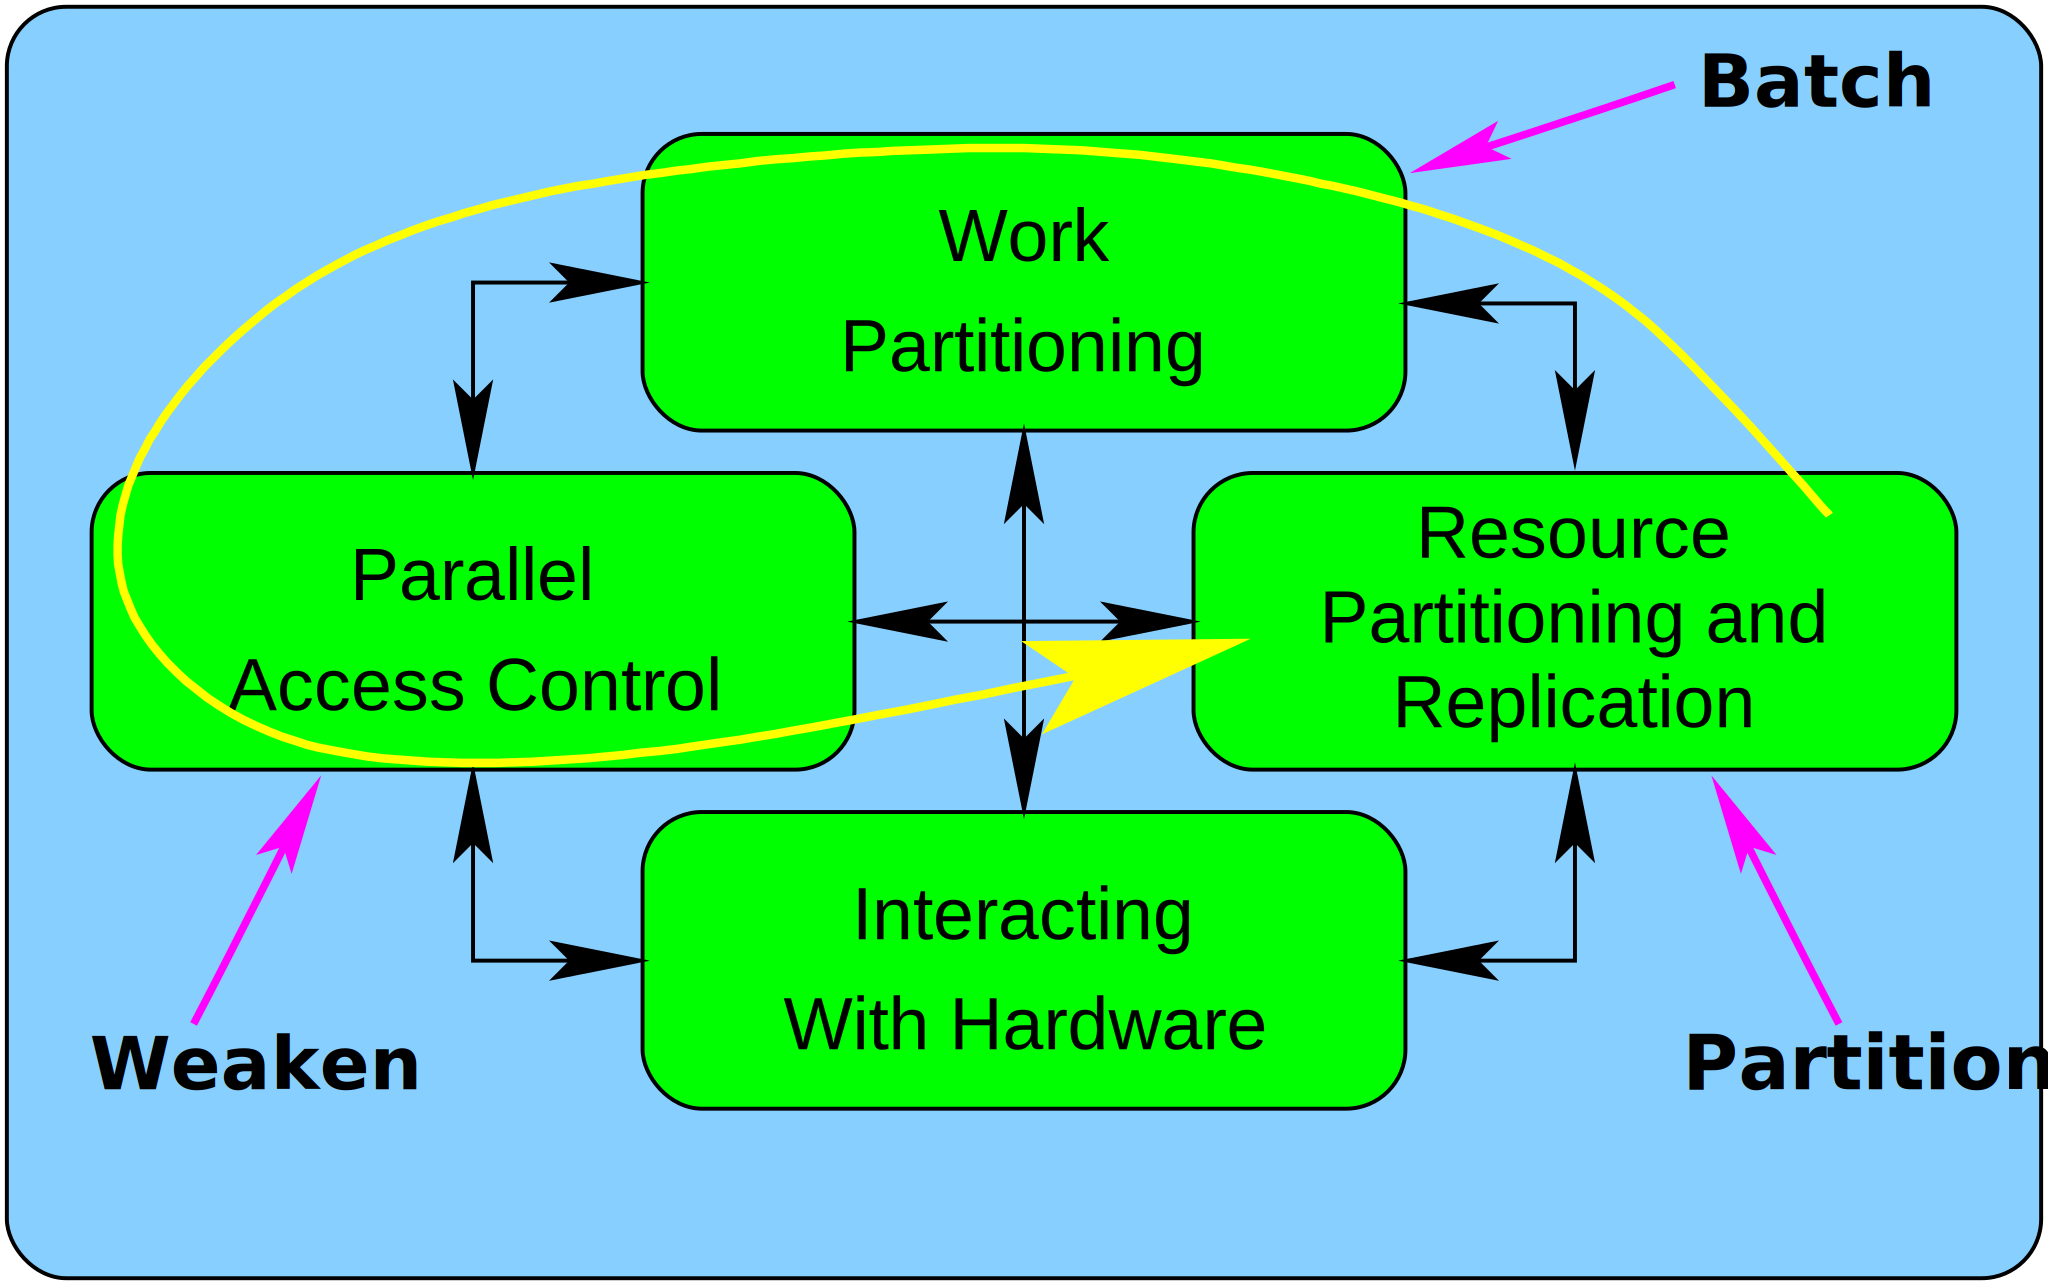
\includegraphics{count/FourTaskOrderOpt}}
\caption{Optimization and the Four Parallel-Programming Tasks}
\label{fig:count:Optimization and the Four Parallel-Programming Tasks}
\end{figure}

Summarizing still further, we have the ``big three'' methods of
increasing performance and scalability, namely
(1)~\emph{partitioning} over CPUs or threads,
(2)~\emph{batching} so that more work can be done by each expensive
synchronization operations, and
(3)~\emph{weakening} synchronization operations where feasible.
As a rough rule of thumb, you should apply these methods in this order,
as was noted earlier in the discussion of
Figure~\ref{fig:intro:Ordering of Parallel-Programming Tasks}
on
page~\pageref{fig:intro:Ordering of Parallel-Programming Tasks}.
The partitioning optimization applies to the
``Resource Partitioning and Replication'' bubble,
the batching optimization to the ``Work Partitioning'' bubble,
and the weakening optimization to the ``Parallel Access Control'' bubble,
as shown in
Figure~\ref{fig:count:Optimization and the Four Parallel-Programming Tasks}.
Of course, if you are using special-purpose hardware such as
digital signal processors (DSPs), field-programmable gate arrays (FPGAs),
or general-purpose graphical processing units (GPGPUs), you may need
to pay close attention to the ``Interacting With Hardware'' bubble
throughout the design process.
For example, the structure of a GPGPU's hardware threads and memory
connectivity might richly reward very careful partitioning
and batching design decisions.

In short, as noted at the beginning of this chapter, the simplicity
of counting have allowed us to explore many
fundamental concurrency issues without the distraction of
complex synchronization primitives or elaborate data structures.
Such synchronization primitives and data structures are covered
in later chapters.
